% **************************************************************************************************************
% A Classic Thesis Style
% An Homage to The Elements of Typographic Style
%
% Copyright (C) 2018 André Miede and Ivo Pletikosić
%
% If you like the style then I would appreciate a postcard. My address
% can be found in the file ClassicThesis.pdf. A collection of the
% postcards I received so far is available online at
% http://postcards.miede.de
%
% License:
% This program is free software; you can redistribute it and/or modify
% it under the terms of the GNU General Public License as published by
% the Free Software Foundation; either version 2 of the License, or
% (at your option) any later version.
%
% This program is distributed in the hope that it will be useful,
% but WITHOUT ANY WARRANTY; without even the implied warranty of
% MERCHANTABILITY or FITNESS FOR A PARTICULAR PURPOSE.  See the
% GNU General Public License for more details.
%
% You should have received a copy of the GNU General Public License
% along with this program; see the file COPYING.  If not, write to
% the Free Software Foundation, Inc., 59 Temple Place - Suite 330,
% Boston, MA 02111-1307, USA.
%
% PLEASE SEE ALSO THE AUTHORS' NOTE REGARDING THIS LICENSE
% IN THE DOCUMENTATION (ClassicThesis.pdf --> Chapter 1 / Chapter01.tex)
% **************************************************************************************************************
\RequirePackage{silence} % :-\
    \WarningFilter{scrreprt}{Usage of package `titlesec'}
    %\WarningFilter{scrreprt}{Activating an ugly workaround}
    \WarningFilter{titlesec}{Non standard sectioning command detected}
\documentclass[ twoside,openright,titlepage,numbers=noenddot,%1headlines,
                headinclude,footinclude,cleardoublepage=empty,abstract=on,
                BCOR=5mm,paper=a4,fontsize=11pt
                ]{scrreprt}

%********************************************************************
% Note: Make all your adjustments in here
%*******************************************************
% ****************************************************************************************************
% classicthesis-config.tex
% formerly known as loadpackages.sty, classicthesis-ldpkg.sty, and classicthesis-preamble.sty
% Use it at the beginning of your ClassicThesis.tex, or as a LaTeX Preamble
% in your ClassicThesis.{tex,lyx} with % ****************************************************************************************************
% classicthesis-config.tex
% formerly known as loadpackages.sty, classicthesis-ldpkg.sty, and classicthesis-preamble.sty
% Use it at the beginning of your ClassicThesis.tex, or as a LaTeX Preamble
% in your ClassicThesis.{tex,lyx} with % ****************************************************************************************************
% classicthesis-config.tex
% formerly known as loadpackages.sty, classicthesis-ldpkg.sty, and classicthesis-preamble.sty
% Use it at the beginning of your ClassicThesis.tex, or as a LaTeX Preamble
% in your ClassicThesis.{tex,lyx} with \input{classicthesis-config}
% ****************************************************************************************************
% If you like the classicthesis, then I would appreciate a postcard.
% My address can be found in the file ClassicThesis.pdf. A collection
% of the postcards I received so far is available online at
% http://postcards.miede.de
% ****************************************************************************************************


% ****************************************************************************************************
% 0. Set the encoding of your files. UTF-8 is the only sensible encoding nowadays. If you can't read
% äöüßáéçèê∂åëæƒÏ€ then change the encoding setting in your editor, not the line below. If your editor
% does not support utf8 use another editor!
% ****************************************************************************************************
\PassOptionsToPackage{utf8}{inputenc}
  \usepackage{inputenc}

\PassOptionsToPackage{T1}{fontenc} % T2A for cyrillics
  \usepackage{fontenc}


% ****************************************************************************************************
% 1. Configure classicthesis for your needs here, e.g., remove "drafting" below
% in order to deactivate the time-stamp on the pages
% (see ClassicThesis.pdf for more information):
% ****************************************************************************************************
\PassOptionsToPackage{
  drafting=true,    % print version information on the bottom of the pages
  tocaligned=false, % the left column of the toc will be aligned (no indentation)
  dottedtoc=false,  % page numbers in ToC flushed right
  eulerchapternumbers=true, % use AMS Euler for chapter font (otherwise Palatino)
  linedheaders=false,       % chaper headers will have line above and beneath
  floatperchapter=true,     % numbering per chapter for all floats (i.e., Figure 1.1)
  eulermath=false,  % use awesome Euler fonts for mathematical formulae (only with pdfLaTeX)
  beramono=true,    % toggle a nice monospaced font (w/ bold)
  palatino=true,    % deactivate standard font for loading another one, see the last section at the end of this file for suggestions
  style=classicthesis % classicthesis, arsclassica
}{classicthesis}


% ****************************************************************************************************
% 2. Personal data and user ad-hoc commands (insert your own data here)
% ****************************************************************************************************
\newcommand{\myTitle}{A Classic Thesis Style\xspace}
\newcommand{\mySubtitle}{An Homage to The Elements of Typographic Style\xspace}
\newcommand{\myDegree}{Doktor-Ingenieur (Dr.-Ing.)\xspace}
\newcommand{\myName}{André Miede \& Ivo Pletikosić\xspace}
\newcommand{\myProf}{Put name here\xspace}
\newcommand{\myOtherProf}{Put name here\xspace}
\newcommand{\mySupervisor}{Put name here\xspace}
\newcommand{\myFaculty}{Put data here\xspace}
\newcommand{\myDepartment}{Put data here\xspace}
\newcommand{\myUni}{Put data here\xspace}
\newcommand{\myLocation}{Saarbrücken\xspace}
\newcommand{\myTime}{June 2018\xspace}
\newcommand{\myVersion}{\classicthesis}

% ********************************************************************
% Setup, finetuning, and useful commands
% ********************************************************************
\providecommand{\mLyX}{L\kern-.1667em\lower.25em\hbox{Y}\kern-.125emX\@}
\newcommand{\ie}{i.\,e.}
\newcommand{\Ie}{I.\,e.}
\newcommand{\eg}{e.\,g.}
\newcommand{\Eg}{E.\,g.}
% ****************************************************************************************************


% ****************************************************************************************************
% 3. Loading some handy packages
% ****************************************************************************************************
% ********************************************************************
% Packages with options that might require adjustments
% ********************************************************************
\PassOptionsToPackage{ngerman,american}{babel} % change this to your language(s), main language last
% Spanish languages need extra options in order to work with this template
%\PassOptionsToPackage{spanish,es-lcroman}{babel}
    \usepackage{babel}

\usepackage{csquotes}
\PassOptionsToPackage{%
  %backend=biber,bibencoding=utf8, %instead of bibtex
  backend=bibtex8,bibencoding=ascii,%
  language=auto,%
  style=numeric-comp,%
  %style=authoryear-comp, % Author 1999, 2010
  %bibstyle=authoryear,dashed=false, % dashed: substitute rep. author with ---
  sorting=nyt, % name, year, title
  maxbibnames=10, % default: 3, et al.
  %backref=true,%
  natbib=true % natbib compatibility mode (\citep and \citet still work)
}{biblatex}
    \usepackage{biblatex}

\PassOptionsToPackage{fleqn}{amsmath}       % math environments and more by the AMS
  \usepackage{amsmath}

% ********************************************************************
% General useful packages
% ********************************************************************
\usepackage{graphicx} %
\usepackage{scrhack} % fix warnings when using KOMA with listings package
\usepackage{xspace} % to get the spacing after macros right
\PassOptionsToPackage{printonlyused,smaller}{acronym}
  \usepackage{acronym} % nice macros for handling all acronyms in the thesis
  %\renewcommand{\bflabel}[1]{{#1}\hfill} % fix the list of acronyms --> no longer working
  %\renewcommand*{\acsfont}[1]{\textsc{#1}}
  %\renewcommand*{\aclabelfont}[1]{\acsfont{#1}}
  %\def\bflabel#1{{#1\hfill}}
  \def\bflabel#1{{\acsfont{#1}\hfill}}
  \def\aclabelfont#1{\acsfont{#1}}
% ****************************************************************************************************
%\usepackage{pgfplots} % External TikZ/PGF support (thanks to Andreas Nautsch)
%\usetikzlibrary{external}
%\tikzexternalize[mode=list and make, prefix=ext-tikz/]
% ****************************************************************************************************


% ****************************************************************************************************
% 4. Setup floats: tables, (sub)figures, and captions
% ****************************************************************************************************
\usepackage{tabularx} % better tables
  \setlength{\extrarowheight}{3pt} % increase table row height
\newcommand{\tableheadline}[1]{\multicolumn{1}{l}{\spacedlowsmallcaps{#1}}}
\newcommand{\myfloatalign}{\centering} % to be used with each float for alignment
\usepackage{subfig}
% ****************************************************************************************************


% ****************************************************************************************************
% 5. Setup code listings
% ****************************************************************************************************
\usepackage{listings}
%\lstset{emph={trueIndex,root},emphstyle=\color{BlueViolet}}%\underbar} % for special keywords
\lstset{language=[LaTeX]Tex,%C++,
  morekeywords={PassOptionsToPackage,selectlanguage},
  keywordstyle=\color{RoyalBlue},%\bfseries,
  basicstyle=\small\ttfamily,
  %identifierstyle=\color{NavyBlue},
  commentstyle=\color{Green}\ttfamily,
  stringstyle=\rmfamily,
  numbers=none,%left,%
  numberstyle=\scriptsize,%\tiny
  stepnumber=5,
  numbersep=8pt,
  showstringspaces=false,
  breaklines=true,
  %frameround=ftff,
  %frame=single,
  belowcaptionskip=.75\baselineskip
  %frame=L
}
% ****************************************************************************************************




% ****************************************************************************************************
% 6. Last calls before the bar closes
% ****************************************************************************************************
% ********************************************************************
% Her Majesty herself
% ********************************************************************
\usepackage{classicthesis}


% ********************************************************************
% Fine-tune hyperreferences (hyperref should be called last)
% ********************************************************************
\hypersetup{%
  %draft, % hyperref's draft mode, for printing see below
  colorlinks=true, linktocpage=true, pdfstartpage=3, pdfstartview=FitV,%
  % uncomment the following line if you want to have black links (e.g., for printing)
  %colorlinks=false, linktocpage=false, pdfstartpage=3, pdfstartview=FitV, pdfborder={0 0 0},%
  breaklinks=true, pageanchor=true,%
  pdfpagemode=UseNone, %
  % pdfpagemode=UseOutlines,%
  plainpages=false, bookmarksnumbered, bookmarksopen=true, bookmarksopenlevel=1,%
  hypertexnames=true, pdfhighlight=/O,%nesting=true,%frenchlinks,%
  urlcolor=CTurl, linkcolor=CTlink, citecolor=CTcitation, %pagecolor=RoyalBlue,%
  %urlcolor=Black, linkcolor=Black, citecolor=Black, %pagecolor=Black,%
  pdftitle={\myTitle},%
  pdfauthor={\textcopyright\ \myName, \myUni, \myFaculty},%
  pdfsubject={},%
  pdfkeywords={},%
  pdfcreator={pdfLaTeX},%
  pdfproducer={LaTeX with hyperref and classicthesis}%
}


% ********************************************************************
% Setup autoreferences (hyperref and babel)
% ********************************************************************
% There are some issues regarding autorefnames
% http://www.tex.ac.uk/cgi-bin/texfaq2html?label=latexwords
% you have to redefine the macros for the
% language you use, e.g., american, ngerman
% (as chosen when loading babel/AtBeginDocument)
% ********************************************************************
\makeatletter
\@ifpackageloaded{babel}%
  {%
    \addto\extrasamerican{%
      \renewcommand*{\figureautorefname}{Figure}%
      \renewcommand*{\tableautorefname}{Table}%
      \renewcommand*{\partautorefname}{Part}%
      \renewcommand*{\chapterautorefname}{Chapter}%
      \renewcommand*{\sectionautorefname}{Section}%
      \renewcommand*{\subsectionautorefname}{Section}%
      \renewcommand*{\subsubsectionautorefname}{Section}%
    }%
    \addto\extrasngerman{%
      \renewcommand*{\paragraphautorefname}{Absatz}%
      \renewcommand*{\subparagraphautorefname}{Unterabsatz}%
      \renewcommand*{\footnoteautorefname}{Fu\"snote}%
      \renewcommand*{\FancyVerbLineautorefname}{Zeile}%
      \renewcommand*{\theoremautorefname}{Theorem}%
      \renewcommand*{\appendixautorefname}{Anhang}%
      \renewcommand*{\equationautorefname}{Gleichung}%
      \renewcommand*{\itemautorefname}{Punkt}%
    }%
      % Fix to getting autorefs for subfigures right (thanks to Belinda Vogt for changing the definition)
      \providecommand{\subfigureautorefname}{\figureautorefname}%
    }{\relax}
\makeatother


% ********************************************************************
% Development Stuff
% ********************************************************************
\listfiles
%\PassOptionsToPackage{l2tabu,orthodox,abort}{nag}
%  \usepackage{nag}
%\PassOptionsToPackage{warning, all}{onlyamsmath}
%  \usepackage{onlyamsmath}


% ****************************************************************************************************
% 7. Further adjustments (experimental)
% ****************************************************************************************************
% ********************************************************************
% Changing the text area
% ********************************************************************
%\areaset[current]{312pt}{761pt} % 686 (factor 2.2) + 33 head + 42 head \the\footskip
%\setlength{\marginparwidth}{7em}%
%\setlength{\marginparsep}{2em}%

% ********************************************************************
% Using different fonts
% ********************************************************************
%\usepackage[oldstylenums]{kpfonts} % oldstyle notextcomp
% \usepackage[osf]{libertine}
%\usepackage[light,condensed,math]{iwona}
%\renewcommand{\sfdefault}{iwona}
%\usepackage{lmodern} % <-- no osf support :-(
%\usepackage{cfr-lm} %
%\usepackage[urw-garamond]{mathdesign} <-- no osf support :-(
%\usepackage[default,osfigures]{opensans} % scale=0.95
%\usepackage[sfdefault]{FiraSans}
% \usepackage[opticals,mathlf]{MinionPro} % onlytext
% ********************************************************************
%\usepackage[largesc,osf]{newpxtext}
%\linespread{1.05} % a bit more for Palatino
% Used to fix these:
% https://bitbucket.org/amiede/classicthesis/issues/139/italics-in-pallatino-capitals-chapter
% https://bitbucket.org/amiede/classicthesis/issues/45/problema-testatine-su-classicthesis-style
% ********************************************************************
% ****************************************************************************************************

% usefull to get a filesystem structure in the document
\usepackage{dirtree}


% ****************************************************************************************************
% If you like the classicthesis, then I would appreciate a postcard.
% My address can be found in the file ClassicThesis.pdf. A collection
% of the postcards I received so far is available online at
% http://postcards.miede.de
% ****************************************************************************************************


% ****************************************************************************************************
% 0. Set the encoding of your files. UTF-8 is the only sensible encoding nowadays. If you can't read
% äöüßáéçèê∂åëæƒÏ€ then change the encoding setting in your editor, not the line below. If your editor
% does not support utf8 use another editor!
% ****************************************************************************************************
\PassOptionsToPackage{utf8}{inputenc}
  \usepackage{inputenc}

\PassOptionsToPackage{T1}{fontenc} % T2A for cyrillics
  \usepackage{fontenc}


% ****************************************************************************************************
% 1. Configure classicthesis for your needs here, e.g., remove "drafting" below
% in order to deactivate the time-stamp on the pages
% (see ClassicThesis.pdf for more information):
% ****************************************************************************************************
\PassOptionsToPackage{
  drafting=true,    % print version information on the bottom of the pages
  tocaligned=false, % the left column of the toc will be aligned (no indentation)
  dottedtoc=false,  % page numbers in ToC flushed right
  eulerchapternumbers=true, % use AMS Euler for chapter font (otherwise Palatino)
  linedheaders=false,       % chaper headers will have line above and beneath
  floatperchapter=true,     % numbering per chapter for all floats (i.e., Figure 1.1)
  eulermath=false,  % use awesome Euler fonts for mathematical formulae (only with pdfLaTeX)
  beramono=true,    % toggle a nice monospaced font (w/ bold)
  palatino=true,    % deactivate standard font for loading another one, see the last section at the end of this file for suggestions
  style=classicthesis % classicthesis, arsclassica
}{classicthesis}


% ****************************************************************************************************
% 2. Personal data and user ad-hoc commands (insert your own data here)
% ****************************************************************************************************
\newcommand{\myTitle}{A Classic Thesis Style\xspace}
\newcommand{\mySubtitle}{An Homage to The Elements of Typographic Style\xspace}
\newcommand{\myDegree}{Doktor-Ingenieur (Dr.-Ing.)\xspace}
\newcommand{\myName}{André Miede \& Ivo Pletikosić\xspace}
\newcommand{\myProf}{Put name here\xspace}
\newcommand{\myOtherProf}{Put name here\xspace}
\newcommand{\mySupervisor}{Put name here\xspace}
\newcommand{\myFaculty}{Put data here\xspace}
\newcommand{\myDepartment}{Put data here\xspace}
\newcommand{\myUni}{Put data here\xspace}
\newcommand{\myLocation}{Saarbrücken\xspace}
\newcommand{\myTime}{June 2018\xspace}
\newcommand{\myVersion}{\classicthesis}

% ********************************************************************
% Setup, finetuning, and useful commands
% ********************************************************************
\providecommand{\mLyX}{L\kern-.1667em\lower.25em\hbox{Y}\kern-.125emX\@}
\newcommand{\ie}{i.\,e.}
\newcommand{\Ie}{I.\,e.}
\newcommand{\eg}{e.\,g.}
\newcommand{\Eg}{E.\,g.}
% ****************************************************************************************************


% ****************************************************************************************************
% 3. Loading some handy packages
% ****************************************************************************************************
% ********************************************************************
% Packages with options that might require adjustments
% ********************************************************************
\PassOptionsToPackage{ngerman,american}{babel} % change this to your language(s), main language last
% Spanish languages need extra options in order to work with this template
%\PassOptionsToPackage{spanish,es-lcroman}{babel}
    \usepackage{babel}

\usepackage{csquotes}
\PassOptionsToPackage{%
  %backend=biber,bibencoding=utf8, %instead of bibtex
  backend=bibtex8,bibencoding=ascii,%
  language=auto,%
  style=numeric-comp,%
  %style=authoryear-comp, % Author 1999, 2010
  %bibstyle=authoryear,dashed=false, % dashed: substitute rep. author with ---
  sorting=nyt, % name, year, title
  maxbibnames=10, % default: 3, et al.
  %backref=true,%
  natbib=true % natbib compatibility mode (\citep and \citet still work)
}{biblatex}
    \usepackage{biblatex}

\PassOptionsToPackage{fleqn}{amsmath}       % math environments and more by the AMS
  \usepackage{amsmath}

% ********************************************************************
% General useful packages
% ********************************************************************
\usepackage{graphicx} %
\usepackage{scrhack} % fix warnings when using KOMA with listings package
\usepackage{xspace} % to get the spacing after macros right
\PassOptionsToPackage{printonlyused,smaller}{acronym}
  \usepackage{acronym} % nice macros for handling all acronyms in the thesis
  %\renewcommand{\bflabel}[1]{{#1}\hfill} % fix the list of acronyms --> no longer working
  %\renewcommand*{\acsfont}[1]{\textsc{#1}}
  %\renewcommand*{\aclabelfont}[1]{\acsfont{#1}}
  %\def\bflabel#1{{#1\hfill}}
  \def\bflabel#1{{\acsfont{#1}\hfill}}
  \def\aclabelfont#1{\acsfont{#1}}
% ****************************************************************************************************
%\usepackage{pgfplots} % External TikZ/PGF support (thanks to Andreas Nautsch)
%\usetikzlibrary{external}
%\tikzexternalize[mode=list and make, prefix=ext-tikz/]
% ****************************************************************************************************


% ****************************************************************************************************
% 4. Setup floats: tables, (sub)figures, and captions
% ****************************************************************************************************
\usepackage{tabularx} % better tables
  \setlength{\extrarowheight}{3pt} % increase table row height
\newcommand{\tableheadline}[1]{\multicolumn{1}{l}{\spacedlowsmallcaps{#1}}}
\newcommand{\myfloatalign}{\centering} % to be used with each float for alignment
\usepackage{subfig}
% ****************************************************************************************************


% ****************************************************************************************************
% 5. Setup code listings
% ****************************************************************************************************
\usepackage{listings}
%\lstset{emph={trueIndex,root},emphstyle=\color{BlueViolet}}%\underbar} % for special keywords
\lstset{language=[LaTeX]Tex,%C++,
  morekeywords={PassOptionsToPackage,selectlanguage},
  keywordstyle=\color{RoyalBlue},%\bfseries,
  basicstyle=\small\ttfamily,
  %identifierstyle=\color{NavyBlue},
  commentstyle=\color{Green}\ttfamily,
  stringstyle=\rmfamily,
  numbers=none,%left,%
  numberstyle=\scriptsize,%\tiny
  stepnumber=5,
  numbersep=8pt,
  showstringspaces=false,
  breaklines=true,
  %frameround=ftff,
  %frame=single,
  belowcaptionskip=.75\baselineskip
  %frame=L
}
% ****************************************************************************************************




% ****************************************************************************************************
% 6. Last calls before the bar closes
% ****************************************************************************************************
% ********************************************************************
% Her Majesty herself
% ********************************************************************
\usepackage{classicthesis}


% ********************************************************************
% Fine-tune hyperreferences (hyperref should be called last)
% ********************************************************************
\hypersetup{%
  %draft, % hyperref's draft mode, for printing see below
  colorlinks=true, linktocpage=true, pdfstartpage=3, pdfstartview=FitV,%
  % uncomment the following line if you want to have black links (e.g., for printing)
  %colorlinks=false, linktocpage=false, pdfstartpage=3, pdfstartview=FitV, pdfborder={0 0 0},%
  breaklinks=true, pageanchor=true,%
  pdfpagemode=UseNone, %
  % pdfpagemode=UseOutlines,%
  plainpages=false, bookmarksnumbered, bookmarksopen=true, bookmarksopenlevel=1,%
  hypertexnames=true, pdfhighlight=/O,%nesting=true,%frenchlinks,%
  urlcolor=CTurl, linkcolor=CTlink, citecolor=CTcitation, %pagecolor=RoyalBlue,%
  %urlcolor=Black, linkcolor=Black, citecolor=Black, %pagecolor=Black,%
  pdftitle={\myTitle},%
  pdfauthor={\textcopyright\ \myName, \myUni, \myFaculty},%
  pdfsubject={},%
  pdfkeywords={},%
  pdfcreator={pdfLaTeX},%
  pdfproducer={LaTeX with hyperref and classicthesis}%
}


% ********************************************************************
% Setup autoreferences (hyperref and babel)
% ********************************************************************
% There are some issues regarding autorefnames
% http://www.tex.ac.uk/cgi-bin/texfaq2html?label=latexwords
% you have to redefine the macros for the
% language you use, e.g., american, ngerman
% (as chosen when loading babel/AtBeginDocument)
% ********************************************************************
\makeatletter
\@ifpackageloaded{babel}%
  {%
    \addto\extrasamerican{%
      \renewcommand*{\figureautorefname}{Figure}%
      \renewcommand*{\tableautorefname}{Table}%
      \renewcommand*{\partautorefname}{Part}%
      \renewcommand*{\chapterautorefname}{Chapter}%
      \renewcommand*{\sectionautorefname}{Section}%
      \renewcommand*{\subsectionautorefname}{Section}%
      \renewcommand*{\subsubsectionautorefname}{Section}%
    }%
    \addto\extrasngerman{%
      \renewcommand*{\paragraphautorefname}{Absatz}%
      \renewcommand*{\subparagraphautorefname}{Unterabsatz}%
      \renewcommand*{\footnoteautorefname}{Fu\"snote}%
      \renewcommand*{\FancyVerbLineautorefname}{Zeile}%
      \renewcommand*{\theoremautorefname}{Theorem}%
      \renewcommand*{\appendixautorefname}{Anhang}%
      \renewcommand*{\equationautorefname}{Gleichung}%
      \renewcommand*{\itemautorefname}{Punkt}%
    }%
      % Fix to getting autorefs for subfigures right (thanks to Belinda Vogt for changing the definition)
      \providecommand{\subfigureautorefname}{\figureautorefname}%
    }{\relax}
\makeatother


% ********************************************************************
% Development Stuff
% ********************************************************************
\listfiles
%\PassOptionsToPackage{l2tabu,orthodox,abort}{nag}
%  \usepackage{nag}
%\PassOptionsToPackage{warning, all}{onlyamsmath}
%  \usepackage{onlyamsmath}


% ****************************************************************************************************
% 7. Further adjustments (experimental)
% ****************************************************************************************************
% ********************************************************************
% Changing the text area
% ********************************************************************
%\areaset[current]{312pt}{761pt} % 686 (factor 2.2) + 33 head + 42 head \the\footskip
%\setlength{\marginparwidth}{7em}%
%\setlength{\marginparsep}{2em}%

% ********************************************************************
% Using different fonts
% ********************************************************************
%\usepackage[oldstylenums]{kpfonts} % oldstyle notextcomp
% \usepackage[osf]{libertine}
%\usepackage[light,condensed,math]{iwona}
%\renewcommand{\sfdefault}{iwona}
%\usepackage{lmodern} % <-- no osf support :-(
%\usepackage{cfr-lm} %
%\usepackage[urw-garamond]{mathdesign} <-- no osf support :-(
%\usepackage[default,osfigures]{opensans} % scale=0.95
%\usepackage[sfdefault]{FiraSans}
% \usepackage[opticals,mathlf]{MinionPro} % onlytext
% ********************************************************************
%\usepackage[largesc,osf]{newpxtext}
%\linespread{1.05} % a bit more for Palatino
% Used to fix these:
% https://bitbucket.org/amiede/classicthesis/issues/139/italics-in-pallatino-capitals-chapter
% https://bitbucket.org/amiede/classicthesis/issues/45/problema-testatine-su-classicthesis-style
% ********************************************************************
% ****************************************************************************************************

% usefull to get a filesystem structure in the document
\usepackage{dirtree}


% ****************************************************************************************************
% If you like the classicthesis, then I would appreciate a postcard.
% My address can be found in the file ClassicThesis.pdf. A collection
% of the postcards I received so far is available online at
% http://postcards.miede.de
% ****************************************************************************************************


% ****************************************************************************************************
% 0. Set the encoding of your files. UTF-8 is the only sensible encoding nowadays. If you can't read
% äöüßáéçèê∂åëæƒÏ€ then change the encoding setting in your editor, not the line below. If your editor
% does not support utf8 use another editor!
% ****************************************************************************************************
\PassOptionsToPackage{utf8}{inputenc}
  \usepackage{inputenc}

\PassOptionsToPackage{T1}{fontenc} % T2A for cyrillics
  \usepackage{fontenc}


% ****************************************************************************************************
% 1. Configure classicthesis for your needs here, e.g., remove "drafting" below
% in order to deactivate the time-stamp on the pages
% (see ClassicThesis.pdf for more information):
% ****************************************************************************************************
\PassOptionsToPackage{
  drafting=true,    % print version information on the bottom of the pages
  tocaligned=false, % the left column of the toc will be aligned (no indentation)
  dottedtoc=false,  % page numbers in ToC flushed right
  eulerchapternumbers=true, % use AMS Euler for chapter font (otherwise Palatino)
  linedheaders=false,       % chaper headers will have line above and beneath
  floatperchapter=true,     % numbering per chapter for all floats (i.e., Figure 1.1)
  eulermath=false,  % use awesome Euler fonts for mathematical formulae (only with pdfLaTeX)
  beramono=true,    % toggle a nice monospaced font (w/ bold)
  palatino=true,    % deactivate standard font for loading another one, see the last section at the end of this file for suggestions
  style=classicthesis % classicthesis, arsclassica
}{classicthesis}


% ****************************************************************************************************
% 2. Personal data and user ad-hoc commands (insert your own data here)
% ****************************************************************************************************
\newcommand{\myTitle}{A Classic Thesis Style\xspace}
\newcommand{\mySubtitle}{An Homage to The Elements of Typographic Style\xspace}
\newcommand{\myDegree}{Doktor-Ingenieur (Dr.-Ing.)\xspace}
\newcommand{\myName}{André Miede \& Ivo Pletikosić\xspace}
\newcommand{\myProf}{Put name here\xspace}
\newcommand{\myOtherProf}{Put name here\xspace}
\newcommand{\mySupervisor}{Put name here\xspace}
\newcommand{\myFaculty}{Put data here\xspace}
\newcommand{\myDepartment}{Put data here\xspace}
\newcommand{\myUni}{Put data here\xspace}
\newcommand{\myLocation}{Saarbrücken\xspace}
\newcommand{\myTime}{June 2018\xspace}
\newcommand{\myVersion}{\classicthesis}

% ********************************************************************
% Setup, finetuning, and useful commands
% ********************************************************************
\providecommand{\mLyX}{L\kern-.1667em\lower.25em\hbox{Y}\kern-.125emX\@}
\newcommand{\ie}{i.\,e.}
\newcommand{\Ie}{I.\,e.}
\newcommand{\eg}{e.\,g.}
\newcommand{\Eg}{E.\,g.}
% ****************************************************************************************************


% ****************************************************************************************************
% 3. Loading some handy packages
% ****************************************************************************************************
% ********************************************************************
% Packages with options that might require adjustments
% ********************************************************************
\PassOptionsToPackage{ngerman,american}{babel} % change this to your language(s), main language last
% Spanish languages need extra options in order to work with this template
%\PassOptionsToPackage{spanish,es-lcroman}{babel}
    \usepackage{babel}

\usepackage{csquotes}
\PassOptionsToPackage{%
  %backend=biber,bibencoding=utf8, %instead of bibtex
  backend=bibtex8,bibencoding=ascii,%
  language=auto,%
  style=numeric-comp,%
  %style=authoryear-comp, % Author 1999, 2010
  %bibstyle=authoryear,dashed=false, % dashed: substitute rep. author with ---
  sorting=nyt, % name, year, title
  maxbibnames=10, % default: 3, et al.
  %backref=true,%
  natbib=true % natbib compatibility mode (\citep and \citet still work)
}{biblatex}
    \usepackage{biblatex}

\PassOptionsToPackage{fleqn}{amsmath}       % math environments and more by the AMS
  \usepackage{amsmath}

% ********************************************************************
% General useful packages
% ********************************************************************
\usepackage{graphicx} %
\usepackage{scrhack} % fix warnings when using KOMA with listings package
\usepackage{xspace} % to get the spacing after macros right
\PassOptionsToPackage{printonlyused,smaller}{acronym}
  \usepackage{acronym} % nice macros for handling all acronyms in the thesis
  %\renewcommand{\bflabel}[1]{{#1}\hfill} % fix the list of acronyms --> no longer working
  %\renewcommand*{\acsfont}[1]{\textsc{#1}}
  %\renewcommand*{\aclabelfont}[1]{\acsfont{#1}}
  %\def\bflabel#1{{#1\hfill}}
  \def\bflabel#1{{\acsfont{#1}\hfill}}
  \def\aclabelfont#1{\acsfont{#1}}
% ****************************************************************************************************
%\usepackage{pgfplots} % External TikZ/PGF support (thanks to Andreas Nautsch)
%\usetikzlibrary{external}
%\tikzexternalize[mode=list and make, prefix=ext-tikz/]
% ****************************************************************************************************


% ****************************************************************************************************
% 4. Setup floats: tables, (sub)figures, and captions
% ****************************************************************************************************
\usepackage{tabularx} % better tables
  \setlength{\extrarowheight}{3pt} % increase table row height
\newcommand{\tableheadline}[1]{\multicolumn{1}{l}{\spacedlowsmallcaps{#1}}}
\newcommand{\myfloatalign}{\centering} % to be used with each float for alignment
\usepackage{subfig}
% ****************************************************************************************************


% ****************************************************************************************************
% 5. Setup code listings
% ****************************************************************************************************
\usepackage{listings}
%\lstset{emph={trueIndex,root},emphstyle=\color{BlueViolet}}%\underbar} % for special keywords
\lstset{language=[LaTeX]Tex,%C++,
  morekeywords={PassOptionsToPackage,selectlanguage},
  keywordstyle=\color{RoyalBlue},%\bfseries,
  basicstyle=\small\ttfamily,
  %identifierstyle=\color{NavyBlue},
  commentstyle=\color{Green}\ttfamily,
  stringstyle=\rmfamily,
  numbers=none,%left,%
  numberstyle=\scriptsize,%\tiny
  stepnumber=5,
  numbersep=8pt,
  showstringspaces=false,
  breaklines=true,
  %frameround=ftff,
  %frame=single,
  belowcaptionskip=.75\baselineskip
  %frame=L
}
% ****************************************************************************************************




% ****************************************************************************************************
% 6. Last calls before the bar closes
% ****************************************************************************************************
% ********************************************************************
% Her Majesty herself
% ********************************************************************
\usepackage{classicthesis}


% ********************************************************************
% Fine-tune hyperreferences (hyperref should be called last)
% ********************************************************************
\hypersetup{%
  %draft, % hyperref's draft mode, for printing see below
  colorlinks=true, linktocpage=true, pdfstartpage=3, pdfstartview=FitV,%
  % uncomment the following line if you want to have black links (e.g., for printing)
  %colorlinks=false, linktocpage=false, pdfstartpage=3, pdfstartview=FitV, pdfborder={0 0 0},%
  breaklinks=true, pageanchor=true,%
  pdfpagemode=UseNone, %
  % pdfpagemode=UseOutlines,%
  plainpages=false, bookmarksnumbered, bookmarksopen=true, bookmarksopenlevel=1,%
  hypertexnames=true, pdfhighlight=/O,%nesting=true,%frenchlinks,%
  urlcolor=CTurl, linkcolor=CTlink, citecolor=CTcitation, %pagecolor=RoyalBlue,%
  %urlcolor=Black, linkcolor=Black, citecolor=Black, %pagecolor=Black,%
  pdftitle={\myTitle},%
  pdfauthor={\textcopyright\ \myName, \myUni, \myFaculty},%
  pdfsubject={},%
  pdfkeywords={},%
  pdfcreator={pdfLaTeX},%
  pdfproducer={LaTeX with hyperref and classicthesis}%
}


% ********************************************************************
% Setup autoreferences (hyperref and babel)
% ********************************************************************
% There are some issues regarding autorefnames
% http://www.tex.ac.uk/cgi-bin/texfaq2html?label=latexwords
% you have to redefine the macros for the
% language you use, e.g., american, ngerman
% (as chosen when loading babel/AtBeginDocument)
% ********************************************************************
\makeatletter
\@ifpackageloaded{babel}%
  {%
    \addto\extrasamerican{%
      \renewcommand*{\figureautorefname}{Figure}%
      \renewcommand*{\tableautorefname}{Table}%
      \renewcommand*{\partautorefname}{Part}%
      \renewcommand*{\chapterautorefname}{Chapter}%
      \renewcommand*{\sectionautorefname}{Section}%
      \renewcommand*{\subsectionautorefname}{Section}%
      \renewcommand*{\subsubsectionautorefname}{Section}%
    }%
    \addto\extrasngerman{%
      \renewcommand*{\paragraphautorefname}{Absatz}%
      \renewcommand*{\subparagraphautorefname}{Unterabsatz}%
      \renewcommand*{\footnoteautorefname}{Fu\"snote}%
      \renewcommand*{\FancyVerbLineautorefname}{Zeile}%
      \renewcommand*{\theoremautorefname}{Theorem}%
      \renewcommand*{\appendixautorefname}{Anhang}%
      \renewcommand*{\equationautorefname}{Gleichung}%
      \renewcommand*{\itemautorefname}{Punkt}%
    }%
      % Fix to getting autorefs for subfigures right (thanks to Belinda Vogt for changing the definition)
      \providecommand{\subfigureautorefname}{\figureautorefname}%
    }{\relax}
\makeatother


% ********************************************************************
% Development Stuff
% ********************************************************************
\listfiles
%\PassOptionsToPackage{l2tabu,orthodox,abort}{nag}
%  \usepackage{nag}
%\PassOptionsToPackage{warning, all}{onlyamsmath}
%  \usepackage{onlyamsmath}


% ****************************************************************************************************
% 7. Further adjustments (experimental)
% ****************************************************************************************************
% ********************************************************************
% Changing the text area
% ********************************************************************
%\areaset[current]{312pt}{761pt} % 686 (factor 2.2) + 33 head + 42 head \the\footskip
%\setlength{\marginparwidth}{7em}%
%\setlength{\marginparsep}{2em}%

% ********************************************************************
% Using different fonts
% ********************************************************************
%\usepackage[oldstylenums]{kpfonts} % oldstyle notextcomp
% \usepackage[osf]{libertine}
%\usepackage[light,condensed,math]{iwona}
%\renewcommand{\sfdefault}{iwona}
%\usepackage{lmodern} % <-- no osf support :-(
%\usepackage{cfr-lm} %
%\usepackage[urw-garamond]{mathdesign} <-- no osf support :-(
%\usepackage[default,osfigures]{opensans} % scale=0.95
%\usepackage[sfdefault]{FiraSans}
% \usepackage[opticals,mathlf]{MinionPro} % onlytext
% ********************************************************************
%\usepackage[largesc,osf]{newpxtext}
%\linespread{1.05} % a bit more for Palatino
% Used to fix these:
% https://bitbucket.org/amiede/classicthesis/issues/139/italics-in-pallatino-capitals-chapter
% https://bitbucket.org/amiede/classicthesis/issues/45/problema-testatine-su-classicthesis-style
% ********************************************************************
% ****************************************************************************************************

% usefull to get a filesystem structure in the document
\usepackage{dirtree}



%********************************************************************
% Bibliographies
%*******************************************************
\addbibresource{Bibliography.bib}
\addbibresource[label=ownpubs]{AMiede_Publications.bib}

%********************************************************************
% Hyphenation
%*******************************************************
%\hyphenation{put special hyphenation here}

% ********************************************************************
% GO!GO!GO! MOVE IT!
%*******************************************************
\begin{document}
\frenchspacing
\raggedbottom
\selectlanguage{american} % american ngerman
%\renewcommand*{\bibname}{new name}
%\setbibpreamble{}
\pagenumbering{roman}
\pagestyle{plain}
%********************************************************************
% Frontmatter
%*******************************************************
%*******************************************************
% Little Dirty Titlepage
%*******************************************************
\thispagestyle{empty}
%\pdfbookmark[1]{Titel}{title}
%*******************************************************
\begin{center}
    \spacedlowsmallcaps{\myName} \\ \medskip

    \begingroup
        \color{CTtitle}\spacedallcaps{\myTitle}
    \endgroup
\end{center}

%*******************************************************
% Titlepage
%*******************************************************
\begin{titlepage}
    %\pdfbookmark[1]{\myTitle}{titlepage}
    % if you want the titlepage to be centered, uncomment and fine-tune the line below (KOMA classes environment)
    \begin{addmargin}[-1cm]{-3cm}
    \begin{center}
        \large

        \hfill

        \vfill

        \begingroup
            \color{CTtitle}\spacedallcaps{\myTitle} \\ \bigskip
        \endgroup

        \spacedlowsmallcaps{\myName}

        \vfill

        
\includegraphics[width=6cm]{gfx/TFZsuperellipse_bw} \\ \medskip

        \mySubtitle \\ \medskip
        %\myDegree \\
        %\myDepartment \\
        %\myFaculty \\
        %\myUni \\ \bigskip

        \myTime\ -- \myVersion

        \vfill

    \end{center}
  \end{addmargin}
\end{titlepage}




% Inizio del Frontespizio

\thispagestyle{empty}
\enlargethispage{60mm}
\begin{center}
\Large{\textsc{Politecnico di Milano}}\\
%\vspace{5mm}
\large{V Facolt\`a di Ingegneria}\\
%\vspace{5mm}
\large{Corso di laurea in Ingegneria delle Telecomunicazioni}\\
\large{Dipartimento di Elettronica e Informazione}\\
\vspace{7mm}
\begin{figure}[h]
\begin{center}

\includegraphics[scale=0.15]{gfx/logo}
\end{center}
\end{figure}
\vspace{2mm}

% titolo della tesi
\begin{LARGE}
TITOLO DELLA TESI
\end{LARGE}
\vspace{25mm}

% relatore
\begin{flushleft}
\begin{tabular}{l l }
Relatore:    & Prof. Nome COGNOME\\
Correlatore: & Ing. Nome COGNOME\\
\end{tabular}
\end{flushleft}
\vspace{25mm}

% autore/autori
\begin{flushright}
\begin{tabular}{l l }
Tesi di Laurea di: & \\
Simone Mosciatti & Matr. 878758
\end{tabular}
\end{flushright}
\vspace{43mm}
{\large{\textbf{ Anno Accademico 2017-2018}}}
\end{center}


\thispagestyle{empty}

\hfill

\vfill

\noindent\myName: \textit{\myTitle,} \mySubtitle, %\myDegree,
\textcopyright\ \myTime

%\bigskip
%
%\noindent\spacedlowsmallcaps{Supervisors}: \\
%\myProf \\
%\myOtherProf \\
%\mySupervisor
%
%\medskip
%
%\noindent\spacedlowsmallcaps{Location}: \\
%\myLocation
%
%\medskip
%
%\noindent\spacedlowsmallcaps{Time Frame}: \\
%\myTime

\cleardoublepage%*******************************************************
% Dedication
%*******************************************************
\thispagestyle{empty}
\phantomsection
\pdfbookmark[1]{Dedication}{Dedication}

\vspace*{3cm}

\begin{center}
    \emph{Ohana} means family. \\
    Family means nobody gets left behind, or forgotten. \\ \medskip
    --- Lilo \& Stitch
\end{center}

\medskip

\begin{center}
    Dedicated to the loving memory of Rudolf Miede. \\ \smallskip
    1939\,--\,2005
\end{center}

%\cleardoublepage\include{FrontBackmatter/Foreword}
\cleardoublepage%*******************************************************
% Abstract
%*******************************************************
%\renewcommand{\abstractname}{Abstract}
\pdfbookmark[1]{Abstract}{Abstract}
% \addcontentsline{toc}{chapter}{\tocEntry{Abstract}}
\begingroup
\let\clearpage\relax
\let\cleardoublepage\relax
\let\cleardoublepage\relax

\chapter*{Abstract}
Short summary of the contents in English\dots a great guide by
Kent Beck how to write good abstracts can be found here:
\begin{center}
\url{https://plg.uwaterloo.ca/~migod/research/beckOOPSLA.html}
\end{center}

\vfill

\begin{otherlanguage}{ngerman}
\pdfbookmark[1]{Zusammenfassung}{Zusammenfassung}
\chapter*{Zusammenfassung}
Kurze Zusammenfassung des Inhaltes in deutscher Sprache\dots
\end{otherlanguage}

\endgroup

\vfill

\cleardoublepage%*******************************************************
% Acknowledgments
%*******************************************************
\pdfbookmark[1]{Acknowledgments}{acknowledgments}

\begin{flushright}{\slshape
    We have seen that computer programming is an art, \\
    because it applies accumulated knowledge to the world, \\
    because it requires skill and ingenuity, and especially \\
    because it produces objects of beauty.} \\ \medskip
    --- \defcitealias{knuth:1974}{Donald E. Knuth}\citetalias{knuth:1974} \citep{knuth:1974}
\end{flushright}



\bigskip

\begingroup
\let\clearpage\relax
\let\cleardoublepage\relax
\let\cleardoublepage\relax
\chapter*{Acknowledgments}
Put your acknowledgments here.

Many thanks to everybody who already sent me a postcard!

Regarding the typography and other help, many thanks go to Marco
Kuhlmann, Philipp Lehman, Lothar Schlesier, Jim Young, Lorenzo
Pantieri and Enrico Gregorio\footnote{Members of GuIT (Gruppo
Italiano Utilizzatori di \TeX\ e \LaTeX )}, J\"org Sommer,
Joachim K\"ostler, Daniel Gottschlag, Denis Aydin, Paride
Legovini, Steffen Prochnow, Nicolas Repp, Hinrich Harms,
Roland Winkler, Jörg Weber, Henri Menke, Claus Lahiri,
Clemens Niederberger, Stefano Bragaglia, Jörn Hees,
Scott Lowe, Dave Howcroft, Jos\'e M. Alcaide, David Carlisle,
Ulrike Fischer, Hugues de Lassus, Csaba Hajdu, Dave Howcroft, 
and the whole \LaTeX-community for support, ideas and
some great software.

\bigskip

\noindent\emph{Regarding \mLyX}: The \mLyX\ port was intially done by
\emph{Nicholas Mariette} in March 2009 and continued by
\emph{Ivo Pletikosi\'c} in 2011. Thank you very much for your
work and for the contributions to the original style.


\endgroup

\cleardoublepage%*******************************************************
% Table of Contents
%*******************************************************
\pagestyle{scrheadings}
%\phantomsection
\pdfbookmark[1]{\contentsname}{tableofcontents}
\setcounter{tocdepth}{2} % <-- 2 includes up to subsections in the ToC
\setcounter{secnumdepth}{3} % <-- 3 numbers up to subsubsections
\manualmark
\markboth{\spacedlowsmallcaps{\contentsname}}{\spacedlowsmallcaps{\contentsname}}
\tableofcontents
\automark[section]{chapter}
\renewcommand{\chaptermark}[1]{\markboth{\spacedlowsmallcaps{#1}}{\spacedlowsmallcaps{#1}}}
\renewcommand{\sectionmark}[1]{\markright{\textsc{\thesection}\enspace\spacedlowsmallcaps{#1}}}
%*******************************************************
% List of Figures and of the Tables
%*******************************************************
\clearpage
% \pagestyle{empty} % Uncomment this line if your lists should not have any headlines with section name and page number
\begingroup
    \let\clearpage\relax
    \let\cleardoublepage\relax
    %*******************************************************
    % List of Figures
    %*******************************************************
    %\phantomsection
    %\addcontentsline{toc}{chapter}{\listfigurename}
    \pdfbookmark[1]{\listfigurename}{lof}
    \listoffigures

    \vspace{8ex}

    %*******************************************************
    % List of Tables
    %*******************************************************
    %\phantomsection
    %\addcontentsline{toc}{chapter}{\listtablename}
    \pdfbookmark[1]{\listtablename}{lot}
    \listoftables

    \vspace{8ex}
    % \newpage

    %*******************************************************
    % List of Listings
    %*******************************************************
    %\phantomsection
    %\addcontentsline{toc}{chapter}{\lstlistlistingname}
    \pdfbookmark[1]{\lstlistlistingname}{lol}
    \lstlistoflistings

    \vspace{8ex}

    %*******************************************************
    % Acronyms
    %*******************************************************
    %\phantomsection
    \pdfbookmark[1]{Acronyms}{acronyms}
    \markboth{\spacedlowsmallcaps{Acronyms}}{\spacedlowsmallcaps{Acronyms}}
    \chapter*{Acronyms}
    \begin{acronym}[UMLX]
        \acro{DRY}{Don't Repeat Yourself}
        \acro{API}{Application Programming Interface}
        \acro{UML}{Unified Modeling Language}
    \end{acronym}

\endgroup

%********************************************************************
% Mainmatter
%*******************************************************
\cleardoublepage
\pagestyle{scrheadings}
\pagenumbering{arabic}
%\setcounter{page}{90}
% use \cleardoublepage here to avoid problems with pdfbookmark
\cleardoublepage
%************************************************
\chapter{Introduction}\label{ch:introduction}
%************************************************

CERN, European Organization for Nuclear Research, (French: Conseil européen
pour la recherche nucléaire) is an European research organization that operates
the largest particle physics laboratory in the world.

Its mission is to:
\begin{itemize}
	\item Provide a unique range of particle accelerator facilities that enable research at the forefront of human knowledge
	\item Perform world-class research in fundamental physics
	\item Unite people from all over the world to push the frontiers of sciences and technology, for the benefits of all.
\end{itemize}

It host the instrument of the 4 biggest physic collaborations: ALICE, ATLAS,
CMS and LHCb.

CERN hosts also a plethora of smaller physic collaborations that benefits from
the instruments, know how, network effects and services available.

Between the services offered to its users the computing service is one of the
most interesting. Indeed CERN hosts and manages the WLCG \cite{grid:website}, one
of the biggest computing data center used for public research.

An issue that affects the operations inside the data center is the provisioning
of software on the computing servers. Scientific software is large and is very
time and bandwidth consuming moving every binaries from a central repository to
the computing nodes.  Several solutions have been proposed and eventually the
problem has been solved with the use of CernVM-FileSystem \cite{cvmfs}, a read
only file-system that provides a scalable, reliable and low maintenance
software distribution system.

However simply provide the servers with the necessary software is not enough.
Indeed also run time dependencies need to be managed to ensure smooth
operations. A possible solution to manage run time dependencies is the use of
containers. Containers pack up all the run time dependencies in an immutable
file system so that they can execute their application always in the same
environment, even if running on different machines. 

However, distribute containers content using CVMFS is not convenient, since the
containers are distributed as a set of big files and this works against the
working principle and performance of CVMFS that works better with a lot of
small files instead of few large files.

This thesis will explore the problem of creating a suitable read-only
file-system structure to provision containers images on computing nodes. We
will provide a general read-only file-system structure and we will implement the
proposed methodology on top of CVMFS.

This thesis is structured as follows:
\begin{itemize} 
        \item Chapter \ref{ch:background} provides the necessary background. It
                start by exploring the computing architecture at CERN, then it
                explain the role of CVMFS, its high level architecture and how
                and why it fits well in the WLCG geographically distributed
                data center. The chapter will then illustrate the container
                run-times that we will exploit in this work and how they
                interact with CVMFS. Finally we are going to state the problem
                definition of this thesis.  
        \item Chapter \ref{ch:SoA} will describe the state of the art. We will
                start by illustrating few distributed file systems and their
                architecture. Then we will move on to describe how provisioning
                of servers is done in environments of different size and
                dimensions.  The last part of this chapter will explore other
                projects in the literature that work lazily as CVMFS.

        \item Chapter \ref{ch:Methodology} will provide the methodology that
                can be used by a generic read-only file system like CVMFS to
                host containers images and achieve efficient content
                distribution.

        \item Chapter \ref{ch:Implementation} will dig into the details of how
                the file system is managed and created on top of CVMFS using
                custom software.

        \item Chapter \ref{ch:Results} will show the result of this work
                comparing start up times of containers in different scenarios
                as well as the bandwidth used.

        \item Chapter \ref{ch:FutureWorks} will finally explore how this work
                can be enhanced and improved. Moreover we will show other
                directions regarding the distribution of containers content
                that we believe are of interest. 
\end{itemize}

\chapter{Background and Problem Definition}\label{ch:background}

In this chapter we are going to introduce the concept and the technologies that
made this work possible.  We will start introducing the Worldwide LHC Computing
Grid (WLCG), which is the \textit{collaboration} that provide the computing power
necessary to the CERN mission. The dimension of the WLCG and its specific
workload required and allowed a specific software distribution system,
CernVM-FileSystem which is used to provision the machines on the WLCG.

Then we will introduce the concept of containers, a different way to solve the
software distribution problem that is widely adopted in the industry. In
particular, we will focus on Docker containers and the Docker images format. We
will then explore Singularity, a container runtime capable of running
containers images stored as simple folder in the file system. Finally we will
explore the Docker \texttt{cvmfs/graphdriver}, a Docker plugin that allow to
run Docker images whose content is available on a read-only file-system without
the need of downloading or accessing the Docker standard images.


\section{WLCG}

The Worldwide LHC Computing Grid is a global collaboration of more than 170
data centers in 42 countries.  The mission of the WLCG is to provide the
computing resources to store, distribute and analyze the data generated by the
operations of the LHC \cite{grid:website},\cite{grid:report}.

The organization of the WLCG follows a hierarchical model, where each level of
the hierarchy is called \textit{Tier}. The most central Tier is the Tier-0,
which is hosted by CERN in the Geneva Area and in Budapest. There are 13 Tier-1
data centers with enough storage and computing capabilities to support the
Grids operation around the clock.  Tiers-1 are geographically distributed: 8 of
them are in Europe, 3 in North America and the rest is in Asia. Finally, the
Tier-2 data centers do not have strict requirements and are generally operated
by research centers and universities \cite{grid:report}.  A schematic
representation of the architecture of the WLCG is provided on Figure
\ref{fig:wlcg-schema}.


\begin{figure}
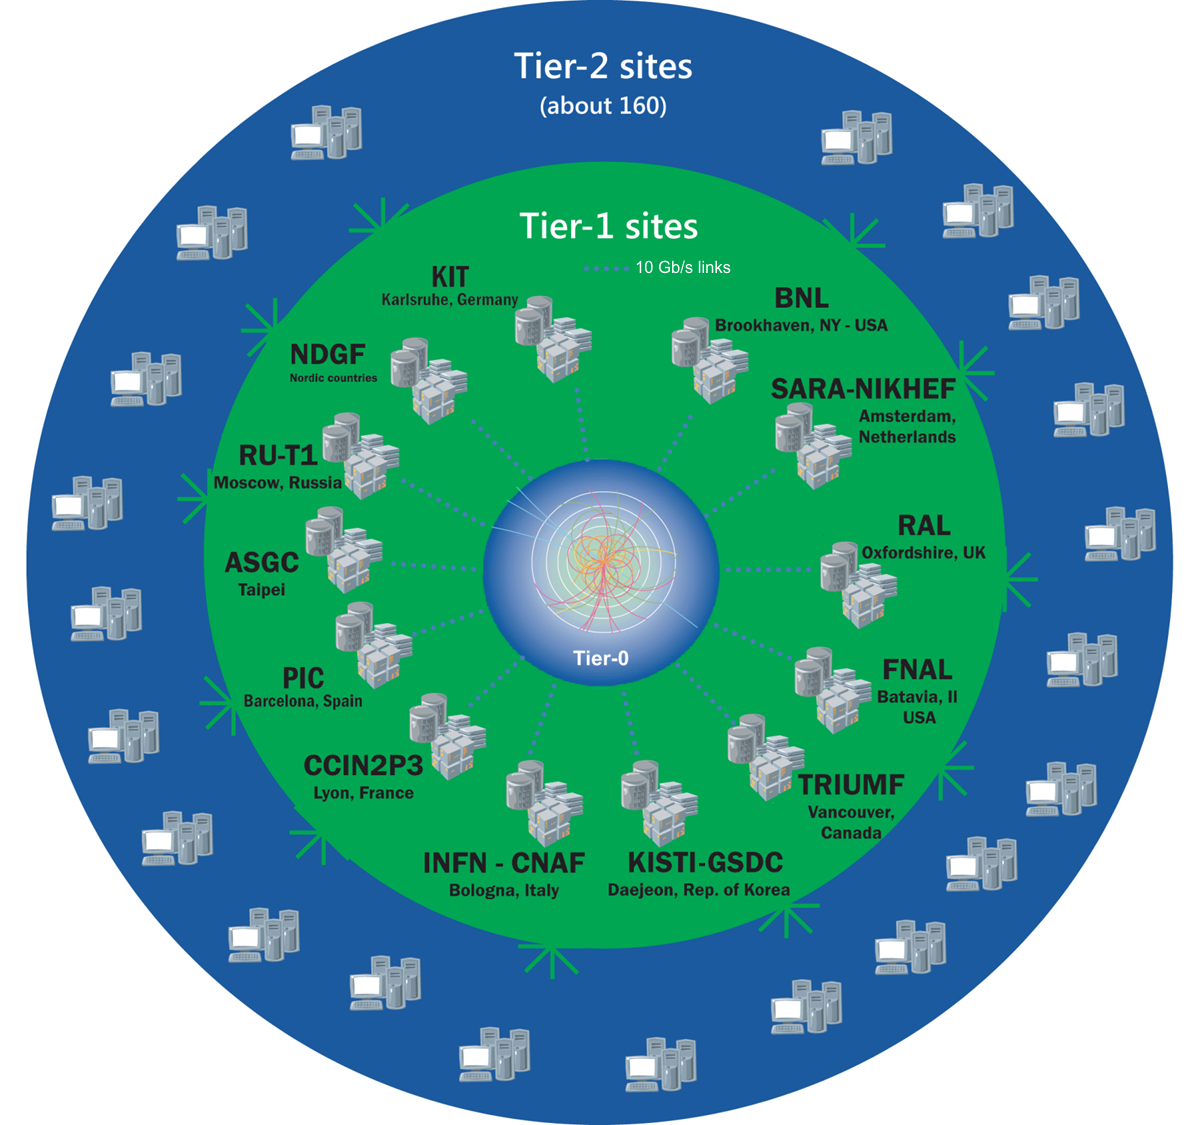
\includegraphics[width=\textwidth,height=\textheight,keepaspectratio]{gfx/WLCG}
\caption{Schematic representation of the WLCG}
\label{fig:wlcg-schema}
\end{figure}

The work of the WLCG is mostly divided in two big classes: analysis of the data
from the LHC detectors and Monte Carlo simulations.  The WLCG assumes and
supports a batch computing paradigm. Analysis and simulations are split in
smaller jobs that are distributed to different computing node that can work in
parallel \cite{grid:report}, \cite{grid:update}.

Before to start each job it is necessary to install the software on the server.
Unfortunately the amount of software potentially needed in each computing node
and the velocity at which the software is updated can make the installation
challenging. Moreover, simpler installation techniques that rely on packages
managers are not applicable since they would put the centralized package
managers themselves under too much load. Several solution have been proposed
and used in the past, eventually it settled for the use of CernVM-FileSystem
(CVMFS) \cite{cvmfs}.

\section{CVMFS} \label{sec:cvmfs}

This section will explore CernVM-FileSystem, we will start with an high level
overview of CVMFS, then we will explore what happens when a file is requested.

\subsection{CVMFS High Level Overview}

CernVM-FileSystem \cite{cvmfs} provides a scalable, reliable and
low-maintenance software distribution system. It is implemented as a read-only
POSIX file-system in user space exploiting FUSE (File-system in USErspace)
\cite{fuse} and standard web server technologies such as Apache or NGNIX.

Each running instance of CVMFS provides a read-only file-system that is
denominated \textit{repository}. At CERN different collaborations maintains
different repositories, but all of them can be mounted from all the computing
node in the WLCG. CVMFS is engineered to support repository of size on the
order of the Terabyte with billions of files.

To save storage space files are addressed by their content (Content Addressable
Storage), hence duplicated files will be stored only once.

In order to distribute software to geographically distant data centers and keep
a low latency, CVMFS allows to cache content in different machines. This allow
to host a cache server in each Tier of the WLCG. The use of caches fits
perfectly with the Tiers model of the WLCG presented above. The Tier-0 host
the main repository (Stratum-0), and the Tier-1 host the first level of cache
(Stratum-1) and so on.

The content of the files are served using the HTTP protocol by a standard
web server. The files are lazily downloaded only on the machine that need them
and only when necessary.

In order to locate and request files from CVMFS the clients download the
catalog, a simple SQLite database which describes a subtree of the whole
file-system.  The catalog contains all the metadata of files and directories,
including owner, group, permission, and size. Moreover the catalog contains
also the URL where to download the files.

A root catalog is available in a know path, and, if the file-system grows too
large, the root catalog links to other sub-catalogs. The use of sub-catalogs
allows to keep each catalog small improving the query time. Moreover, while
normal files hosted in CVMFS can be split into small blocks and each block can
be serve separately, this is not supported for catalogs. Indeed each
sub-catalog needs to be fully downloaded before it can be used. Hence big
catalogs can be a bottleneck both with the respect of query time, download time
and bandwidth.

\subsection{CVMFS Details}\label{subsec:cvmfs-details}

CVMFS is implemented using the Client-Server architecture. The server is
responsible to manage the content of the repository and to expose it via HTTP
API.  The client is installed in the host machine and is responsible to expose
the content of the repository to the users and it is implemented as a FUSE
daemon which implements all the system calls necessary for a read-only
file-system.

When a CVMFS file-system is mounted, it starts by reading a configuration file
which describes each repository. The client then downloads a simple text file
which points to the catalog of the repository. Once the catalog is downloaded
the client has all the information necessary to start responding to the system
calls performed by the user.

As an example, when the user requires a \texttt{stat} system call against a
file, the client reads from the catalog all the information about the file
like, size, permission, mode, etc.. and replies with them. Instead when the
user requires to read from a file, the client first downloads the file from the
server, stores it into a local cache and passes through each read operation to
the local copy.

This approach allows to download only the file really required, since all the
other system calls can be served by just reading from the catalog. However this
implies that the reading latency from a file depends on the network latency.
This strategy works very well if the reading latency of a file is not a major
concern and if reading from the catalog is fast. However, if the catalog grows
too big, then the queries become too slow. 

To overcome this limitation the sub-catalogs were introduced.  A sub-catalog is
exactly like the normal catalog, but while the catalog refers to the whole
file-system tree, a sub-catalog refer to a smaller sub tree of the file-system.
In order to avoid confusion, we will refer to the root-catalog as the catalog
that includes the root of the file-system and to sub-catalog to all the other
catalogs in the file-system. The root-catalog, of course, embeds several
sub-catalogs, and each sub-catalog can, recursively, embed another sub-catalog.

When it is required to read information about a file, the client starts by
looking into the root catalog and then it follows the sub-catalogs structure
until it finds the required file.

\section{Containers}
\label{sec:containers}

While CERN solved its problems of software distribution with CVMFS the industry
opted for a different approach: containers. 
Containers are a standard units of software that package up code and all its
dependencies so that computer applications run quickly and reliably from one
computing environment to another \cite{docker:what}.

In order to standardize containers and make the technology interoperable in
2015 the \textit{Open Container Initiative (OCI)} was founded \cite{oci}. The
OCI defined a standard format to use to pack containers into \textit{images}
\cite{oci:image-spec}, this format have been adopted by Docker and is used in
the \textit{Docker Images}.  A Docker image is an immutable set of tar files,
where each tar file is called layer. Prior to run the container, each layer
gets mounted one on top of the other to re-create the original environment
where to run the application \cite{oci:image-filesystem}. The content of each
image is codified in a \texttt{json} file, the manifest, which provides the
unique name of the image itself and which refers to each layer that compose the
image by their unique identifiers. The unique identifier of both images and
layers is the result of the function \texttt{hash256} of their content
\cite{oci:content}. 

Docker images are distributed through Docker registries, simple HTTP servers
that given the unique identifiers of a layer provide the layer itself,
similarly, given the identifier of an image the registries provides its
manifest \cite{docker:registry}.

Docker allow to associate a human readable identifier to each image, this name
is composed by a namespace, which identifies the user or organization that created
the image, a name, which identifies the image itself and a tag, which identifies
the version of the image. These names are not immutable and are meant to be
used just by humans to recognize and use the images \cite{docker:tag}.
The repository where the image is hosted, its namespace, its name and its tag
create a hierarchical structure between the several images that is easy to
navigate for humans.

\subsection{Docker and the cvmfs/graphdriver plugin}
\label{subsec:docker-thin-images}

Docker is a thin CLI layer on top of a Linux daemon, \texttt{dockerd} which is
responsible to obtain the Docker images from the registries, mount the layers,
manage the runtime of the image and allow communication of a Docker runtime
with the host system \cite{docker:overview}.

Docker layers can be shared between different images, so the Docker daemon
download them once and store them in the local machine for future use
\cite{docker:storage}. On average less than 7\% of the content inside a Docker
image is used during the runtime of the image \cite{slacker}. The layers are
distributed as a single tar file \cite{oci:image-filesystem}, hence a naive
distribution of layers with CVMFS would not provide any advantage. The whole
tar files would need to be downloaded erasing the advantages of using CVMFS.

A solution to this problem was introduced with the \texttt{cvmfs/graphdriver}
plugin and the concept of "thin-images" \cite{graphdriver-plugin}. In this work
we are not interested in the internals of the \texttt{cvmfs/graphdriver} plugin,
it will be sufficient to know that the Docker daemon can be enhanced with the
use of plugins \cite{docker:plugin} and that the plugin allows us to run what
are called "thin-images".

\textit{Thin-images} are Docker images that are created starting from standar
(\textit{fat}) Docker images. The content of a \textit{thin-image} is only a
simple \texttt{json} file whose content is the list of layers needed by the
original \textit{fat-image} and where to find them in the host file-system, we
call this file the \textit{recipe} an example of \textit{recipe} file is show
on Listing \ref{lst:thin-example}. \textit{Thin-images} can be executed only if
the Docker daemon have enabled the \texttt{cvmfs/graphdriver} plugin, indeed
the plugin is able to read the content of the thin-image, mount the original
layers inside the container, and finally execute the application
\cite{graphdriver-plugin}.

\begin{minipage}{\linewidth}
\begin{lstlisting}[caption={Example of a \textit{recipe} file of a Docker \textit{thin image}},label={lst:thin-example}]
{
  "version": "1.0",
  "origin": "https://registry.hub.docker.com/library/python:latest",
  "layers": [
    {
      "digest": "bc9ab7...0257b7",
      "url": "cvmfs://thin.osg.cern.ch/.layers/bc/bc9ab7...0257b7/layerfs"
    },
    {
      "digest": "193a63...110d7f",
      "url": "cvmfs://thin.osg.cern.ch/.layers/19/193a63...110d7f/layerfs"
    },
    {
      "digest": "e5c3f8...818580",
      "url": "cvmfs://thin.osg.cern.ch/.layers/e5/e5c3f8...818580/layerfs"
    },
    {
      "digest": "b61a0d...b615a9",
      "url": "cvmfs://thin.osg.cern.ch/.layers/b6/b61a0d...b615a9/layerfs"
    }
  ]
}
\end{lstlisting}
\end{minipage}



If the files necessary to run the \textit{thin-images} are distributed by CVMFS, it is
possible to run docker containers without downloading any unnecessary content.

Moreover the \texttt{cvmfs/graphdriver} plugin is able to run standard (\textit{fat})
Docker images, hence conventional Docker images are supported seamlessly \cite{graphdriver-plugin}.

On Figure \ref{fig:flowchart-run-thin-image} we show how the plugin decides how
to mount the container file system. If it detects that the image is a standard
\textit{fat} Docker image it runs it as a standard image, if it detects that is a
\textit{thin} image it mounts the layers from the CVMFS read-only file system.

\begin{figure}
\begin{center}
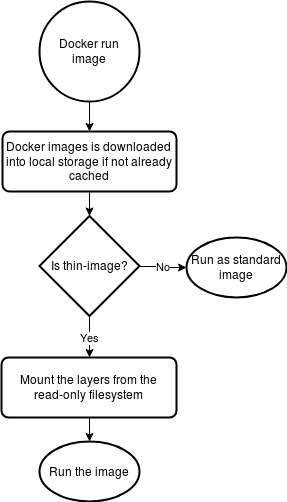
\includegraphics[scale=0.5]{gfx/RunThinImages}
\end{center}
\caption{Decision proces for running docker thin images}
\label{fig:flowchart-run-thin-image}
\end{figure}

The downside of this approach is that a "thin-image" can be downloaded, stored in
the local storage and successfully run using the content provide by CVMFS. On a
second moment the images can be updated, uploaded newly on the registry and the
old content in CVMFS is deleted to host the new content of the image. If now
the user tries to run the same images, it will not download it again from the
registry but it will use the image already cached, referring
to content not available anymore on CVMFS, hence it will fail to run.

\subsection{Singularity}\label{subsec:singularity}

Singularity \citep{singularity:home} is another container runtime, it provides
its own image format but it is capable to run standard Docker images
\cite{singularity:docker} as well.  Moreover it is capable of running
containers, also Docker containers, directly from a directory containing the
unpacked container file-system itself \cite{singularity:run}.

Given the Singularity capability to run Docker containers directly from a
directory containing the unpacked Docker image file-system its integration with
CVMFS is simpler that the one with Docker itself. Indeed it is sufficient to
host the directory containing the unpacked file-system of the Docker image in
CVMFS.

\section{Problem Definition}\label{sec:problem}

We have introduced how CERN has overcome the challenges of software distribution
using CVMFS. Unfortunately this is not enough since run-time dependencies
between software components can break applications that instead are running
perfectly fine in a different environment.

Since containers pack up all their runtime dependencies in a standard
environment they are a suitable solution for this problem. However, containers
are distributed as big tar files which is against the design, working
principles and performance characteristics of CVMFS.

Both CVMFS and containers aim to solve the same challenge of server
provisioning, however they made different trade-offs. CVMFS opted for an
efficient distribution of the content, making difficult and
inconvenient to pack all the runtime dependencies of a particular application.
Containers, instead, opted to make each application self-contained so that the
application can run reliably on different computer environments, however
losing efficiency in the distribution of the content.

Efficient content distribution and efficient dependency management should not
be contrasting goals. For this reason, in this thesis work we will tackle the
problem of how to efficiently distribute software in HPC clusters while
efficiently preserving all its runtime dependencies.



\clearpage
%************************************************
\chapter{State of the Art}\label{ch:SoA}
%************************************************

Other than the distribution of content, CERN faced the problem of managing
run-time dependencies. A possible solution to this problem would be to
statically link all the dependencies, but this would generate extremely big
binaries.  Another solution would be to carefully managing the all the software
installed on the machine, including all the recursive dependencies. However this
clash with the WLCG model where jobs can migrate from a data center to another
along with their dependencies.  Moreover sometimes even a very careful
installation is not sufficient since is possible that two application that
could run on the same machine have clashing dependencies.

The problem of how to manage runtime dependency is been solved outside CERN in
several different way.

On small scale is possible to use simple package managers that automatically
install the dependencies, however they suffer of few different problem. First
and foremost in case of dependencies clashing the package manager simply refuse
to install the required package, which is not an acceptable solution. Then at
the scale of the WLCG the package manager quickly become a bottleneck with the
respect of the bandwidth necessary to distribute the content but also with the
respect of the size of the internal databases.

Another possible solution is the use of containers. Packaging all the runtime
dependencies along the application code in an immutable file system allow
containers to exactly reproduce the same environment and condition to ensure
smooth operations. The use of containers however is not convenient in very
large clusters like the WLCG, indeed the content necessary to run a container
is distribute as few large tar files and this makes the distribution itself
inefficient since a lot of content not useful for the application itself is
downloaded anyway. 

Several system have been propose to decrease the downloading time of containers
images, however all of them work \textit{ahead of runtime} trying to optimize
for how fast the overall system is capable of delivering the whole image into
the host. FID (Faster Image Distribution) \cite{FID} is a P2P Docker images
distribution system that is able to accelerate the speed of distributing Docker
images by taking full advantage of the bandwidth of not only the Docker
Registry but also of the other nodes in the cluster, while decreasing the
downloading time FID still require to download all the image before to run the
computation. Another work by Anwar et all. \cite{210500} characterize the
workload of large-scale registries in order to derive design implication for
more optimize registries, still they are working to optmize the time necessary
to serve and download the whole image from the registry.

While the aim of this work is still to decrease the start up time of uncached
containers we took a different road. While the previous works focus on optimize
the delivering time of the whole content image we decide to focus on minimize
the amount of content that the client needs to download which of course lead to
shorter start up time for the containers and also on saving bandwidth.

Few other system have been proposed to address the problem using a similar
architecture. The \textit{cvmfs/graphdriver} \cite{graphdriver-plugin} allows
us to run Docker images starting from a \textit{recipe} file that  list the
layers to mount and their location in the file system. Unfortunately a way to
provide the \textit{thin images} was not provided, moreover it wasn't provide a
way to structure the file system itself. Slacker \cite{slacker} tackle the same
problem but it use a very different implementation. Their work is based on NFS
and flatten layers. All the layer of an image get flatten into a single layer,
and such layer stored as a single file into a NFS shared between the Docker
Registries and the Docker Client. While \textit{cvmfs/graphdriver} share a set
of layers as Docker images, Slacker share a simple reference to the file stored
in the NFS. Slacker is able to reach very interesting performance thank to the
implementation of the NFS they use that relies on network disks. We lack the
details about the NFS used by Slacker (Tintri 620) but we believe that their
performance may be strongly influenced by the size of the cluster.

In this work we aim to finally bridge the two world of containers and
distributed read-only file system like CVMFS.



\clearpage
%************************************************
\chapter{Problem Definition}\label{ch:ProblemDefinition}
%************************************************

In the Background on chapter \ref{ch:background} we addressed how CERN has
overcome the challenge of software distributions using CVMFS. Unfortunately
this is not enough since run-time dependencies between software components can
break application that instead are running perfectly fine in a different
environment.

A possible solution to this problem is the use of container technology and we
explore how both Singularity and Docker with the \texttt{cvmfs/graphdriver}
plugin are capable to run Docker images hosted in CVMFS avoiding to download
unnecessary from remote host saving bandwidth.

In this work we aim to introduce a read-only file-system structure
implementable in CVMFS that will allow us to bridge together the efficient
content distribution provide by CVMFS with the encapsulation of runtime
dependencies provide by container technologies.

This work will focus on a specific container technology, Docker. Indeed we
focus on describe a file-system structure suitable to run Docker images using
Singularity and the thin-images Docker graphdriver plugin.

The proposed file-system structure aims to the following goals:
\begin{itemize}
\item Minimize the amount of space required
\item Minimize the start up time of containers
\item Minimize the time necessary to add a new docker image into the file-system
\item Minimize the number of files in the CVMFS sub-catalogs 
\item Minimize the complexity of managing the files-ystem itself
\item Provide a great usability for the users.
\end{itemize}

Some of those goal can be measured to asses if we were successful or not, in
particular we are going to:

\begin{itemize}
\item Compare the amount of space required by the CVMFS repository versus the
        amount of space required for each layer.
\item Compare the start-up time of containers hosted in CVMFS versus the
        start-up time of containers not hosted on CVMFS
\item Provide the distribution of number of files in each sub-catalog
\item Measure the complexity of managing the file-system using as a proxy the
        cyclomatic complexity of the software that actually create and manage
                the file-system.
\end{itemize}

Unfortunately we didn't find usable proxy for measuring the usability of the
file-system structure nor it make sense to measure the time necessary to add a
new Docker image into the file-system since it depends on too many variable to
provide a useful measure.

\clearpage
%************************************************
\chapter{Methodology}\label{ch:Methodology}
%************************************************

In this chapter we will introduce a read-only file-system structure for
running Docker images using both Singularity and the docker thin-images plugin.
We focus on Singularity because it is a widely deployed system in HPC and on
Docker thin-images because it allows the user to leverage the Docker infrastructure
to run images whose content is distributed with a read only file-system.

Section \ref{sec:methodology-high-level} will provide a high level overview of
the proposed methodology explaining why we decided to focus our design on CVMFS,
Singularity and Docker with the \textit{cvmfs/graphdriver} plugin.

Section \ref{sec:methodology-singularity} will analyze the file-system
structure to host the Docker images to run with Singularity. We will explain
how we created a hierarchical structure similar to the one of the docker
registries while keeping the repository maintainable and without putting too
much pressure in the sub-catalog system of CVMFS.

Section \ref{sec:methodology-docker} will analyze how we stored the content used
by the thin-images Docker plugin. Structural similarities between Docker images
and Docker layers will drive us to adopt a very similar solution to avoid
stressing the sub-catalog system. The sharing of layers between different
docker images will allow us to avoid repeating work, but it will introduce
difficulties during the deletion of the image itself that we will solve using a
reference count system.

Finally Section \ref{sec:methodology-keep-track} will show how we kept
track of the images already present in the file-system.

\section{High Level overview of the proposed file system}
\label{sec:methodology-high-level}

The aim of this work is to provide an efficient content distribution
system to run containerized application on big distributed clusters.  

The aim of this work is to efficiently distribute software in HPC clusters
while efficiently preserving its runtime dependencies. To tackle this problem
we will resort on CVMFS to efficiently distribute the content of the containers
together with containers technologies to preserving the runtime dependencies in
such a way that only the strictly necessary files will be downloaded into the
worker nodes of the clusters.


The content distribution part will be managed by CVMFS which provides
the primitives necessary to efficiently distribute the content. Moreover, to
the best of our knowledge, CVMFS is the only stable and tested system that
allows to distribute lazily and efficiently Terabytes of data in a distributed
data center like the WLCG.  Starting from the data distributed by CVMFS, there
are two container run-times that we can use to actually run the containers.
The first one is Singularity, introduced in Section \ref{subsec:singularity}
that allows to run containers whose content is already unpacked in a simple
folder. The second one is Docker with the \textit{cvmfs/graphdriver} plugin,
which allows Docker to run \textit{thin images} made of a simple
\textit{recipe} \texttt{json} file which describes where are in the file system
the necessary layers that are needed to be mounted before to start the
container itself.

The proposed structure is absolutely generic and even if not implemented with
CVMFS it would allow the above container run-times to work with minimal
modifications \footnote{The implementation of \textit{cvmfs/graphdriver} relies
on a specific \textit{cvmfs} url in the \textit{recipe} format which is a
simple implementation details that can be easily generalized.}. However some
choices of the directory structures have been taken starting from the design of
CVMFS and may not be necessary on a generic read-only file system.

The proposed file-system provides two main structure. A non-hidden set of
directories that host the unpacked images to run with Singularity and a hidden
folder to host the layers used by the \texttt{cvmfs/graphdriver} Docker plugin.
Along with these structures another hidden directory will contain metadata
information about the Docker images already in the repository.

The directories that host the unpacked Docker images have the same hierarchical
structure of the Docker structure mentioned in Section \ref{sec:containers}, hence
the first directory is the name of the registry that host the image, it follows
the namespace which refers to the user of the organization responsible for the
image and the last level is the image name along with the tag.

The directory that host the layers of the Docker images can conceptually be a
flat structure simply containing the layers each identified by its digest.
However a simple flat structure will put too much pressure in the catalog
system so we aggregated layers that share the same digest prefix and create
a sub-catalog for each aggregation.

The hidden metadata folder will follow the same hierarchical structure of
Docker images, allowing to quickly locate the metadata information of an image
given just the name of the image itself.

\begin{figure}
\dirtree{%
.1 /cvmfs/unpacked.cern.ch.
.2 registry.hub.docker.com.
.3 library.
.4 centos:centos7.
.2 .layers/.
.2 .metadata/.
}
\caption{High level visualization of the proposed file-system}
\label{fig:high-level-fs}
\end{figure}


\section{Singularity Images}
\label{sec:methodology-singularity}

To run Docker images using Singularity it is sufficient to start the singularity
executable providing as input the directory where the image is been unpacked.
In this section we are going to show how we structure the file-system in a way
that allow users to easily discover and run unpacked docker images using
Singularity while keeping the file-system easy to maintain.

As mentioned in Section \ref{sec:containers} Docker images have
a hierarchical structure.  The first level of the hierarchy is the docker
registry where the image is hosted.  The most common registries in our case are
the official docker hub \footnote{\texttt{registry.hub.docker.com}} and the
CERN internal registry \footnote{\texttt{gitlab-registry.cern.ch}}.

The second level in the hierarchical structure is the namespace of the docker
image.  If the image is one of the official docker images it will be the
standard namespace: “library”.  In all the other cases, the namespace will be
the same as the original docker image.  For example for the images belonging to
the ATLAS collaboration we use the namespace \texttt{atlas}.

The last level is the name of the image itself together with the tag of such
image, separated by a colon (\texttt{:}).  We decided to avoid yet another
level containing just the tags.  Indeed there are relatively few tags for each
image and adding another level of indirection would have made it harder to
explore the file-system.  Moreover, we decided to use the colon because it is
the same character used in the docker registries between the images and the tag
and it is immediately recognizable by the users.

\begin{figure}
\dirtree{%
.1 /cvmfs/unpacked.cern.ch.
.2 registry.hub.docker.com.
.3 library.
.4 centos:centos7 -> /cvmfs/unpacked.cern.ch/.flat/75/75835...0c4ab6d.
.4 centos:latest -> /cvmfs/unpacked.cern.ch/.flat/75/75835...0c4ab6d.
.4 debian:stable -> /cvmfs/unpacked.cern.ch/.flat/a4/a4274...ba594cb.
.4 gcc:latest -> /cvmfs/unpacked.cern.ch/.flat/ce/ceccd...a75dd28.
.4 openjdk:9 -> /cvmfs/unpacked.cern.ch/.flat/5a/5adaf...5344d70.
.4 python:2.7 -> /cvmfs/unpacked.cern.ch/.flat/3c/3c43a...0e7c9d4.
.4 python:3.4 -> /cvmfs/unpacked.cern.ch/.flat/43/43953...ed73435.
.3 efajardo.
.4 docker-cms:tensorflow -> /cvmfs/unpacked.cern.ch/.flat/2d/2d5b4...97d44fc.
}
\caption{Visualization of the Filesystem structure, the arrows indicate symbolic links}
\label{fig:simple-fs}
\end{figure}

While this structure is user friendly, it makes the maintenance of the
repository complex.

The tags used in each image are not immutable, hence, without continuous
maintenance, it may happen that the images stored inside the file-system are
not up to date making difficult for the user to know what version of the
software is being run.  Moreover with the described structure, it would be
extremely complex to detect if an image is up to date or if it needs further
updates.

To work around this issues we exploited the fact that each image is uniquely
identified by its digest.  Indeed we decided to store the real content of the
images in an hidden folder that embed the digest itself while preserving the
structure presented above using symbolic links.

We show the directory structure of the file-system on Figure
\ref{fig:simple-fs}.

The folder that contains the real content of a Singularity image are all below
the standard subdirectory \texttt{.flat/}.  The name \texttt{.flat/} was chosen
to make it clear that only flatted file systems are stored in there.

Embedding the digest in the name of the folder allows to immediately find the
location of an image, which is useful when an image become obsolete and need to
be deleted from the file-system.

From a theoretical point of view it would be sufficient to store the whole
content of the Singularity images in the folder \texttt{.flat/\$image\_digest}.
However, from a practical point of view this would create too much content in a
single folder putting too much pressure in the CVMFS sub-catalog system.

To overcome this issue we decided to create a fixed number of
"super-directories" where we placed the unpacked folder of the images.  To
easily locate each unpacked folder in the super-directories we decided to call
each super-directory as the prefix of the digest of the images it is
containing. Since the digest is an hexadecimal string this approach provides us
with $16 \times 16 = 256$ fixed super-directories inside the \texttt{.flat/}
directory, each of which will contain only the content of the images whose
digest start with those 2 specific bytes.

\begin{figure}
\dirtree{%
.1 /cvmfs/unpacked.cern.ch/.flat.
.2 0c.
.3 0cbf37812bff083eb2325468c10aaf82011527c049d66106c3c74298ed239aaf.
.2 2c.
.3 2cc378c061f7b3e8d9096728eb75722a89f31fb3f3117ed10c66cc2f4b8ab281.
.2 5a.
.3 5adaf00da2a3cf6b611e7c850778fad3dc62c548864706b822b5f3ce65344d70.
.2 ea.
.3 ea4c82dcd15a33e3e9c4c37050def20476856a08e59526fbe533cc4e98387e39.
.3 eadfca9546a132104b8bdb6b76952c6e5d412301704b7bc94e9176bcc5dda0fe.
}
\caption{Visualization of the "super directories" in the ".flat" subdirectory}
\label{fig:super-directories}
\end{figure}

On figure \ref{fig:super-directories} we can see that “0c”, “2c”, …, “ea” are
all “super-directories” and each one contains only the file-systems that start
with “0c”, “2c”, …, “ea” respectively.  Note the case of “ea” that contains
file-systems of multiple images whose digest start with “ea”.

However, to relieve pressure from the catalog system is not sufficient to
simply aggregate the images into "super-directories", we also need to create a
sub-catalog for each "super-directory." Moreover, since each image can contains
itself a lot of files we decided to create a sub-catalog also for each unpacked
image.

Another positive side-effect of the use of symbolic links is that symbolic
links manipulation is defined as atomic in the POSIX standard.

The use of "super-directories" is necessary for limits in the implementation of
CVMFS and they are not necessary on an abstract read-only file-system.

\section{Docker Thin Images}
\label{sec:methodology-docker}

While for running docker images using Singularity it is sufficient to have the
image unpacked in a simple directory, running Docker containers using the
thin-images plugin requires a more complex set up.  As explained in Section
\ref{subsec:docker-thin-images} the recipe of the docker thin-image contains
the path of the directories where each layer of the original docker image is
hosted, those directories will be mounted by the docker plugin.

All the docker layers are stored under a common subdirectory of the
file-system, the \texttt{.layers/} directory.

Since the sub-tree of the file-system used by the Docker thin-images is used only
by the Docker plugin we don't need to create a human-friendly structure like we
did for the Singularity sub-tree.

Like docker images also the docker layers are identified by an unique digest,
and similarly to the docker images, store all of them in a single directory
will put too much pressure in the CVMFS sub-catalog system, hence we follow the
exact same model used for storing the unpacked images also for the layers,
creating 216 super-directories.

A big advantage of the use of layers over flat images is that layers can be
shared by multiple images.

The sharing of layers allow us to avoid re-doing work that is already been
done, in particular if a layer is already in the file-system it will not be
added again. On the other hand it makes more complex removing an image since it
is necessary to remove each layer that compose the image, but some layers may be
shared between images.

Removing layers has the important implication that once the layer is removed
every thin image that relies on it would not work anymore.  However those
thin-images could be stored on the client side where we don’t have any access.

To not disrupt the user workflow while keeping the repository to a manageable
size we considered several options: 
\begin{enumerate}
\item Never remove layers
\item Remove layers as soon as possible
\item Provide a grace period before finally removing the layer
\end{enumerate}

The option to never remove layers is impractical since the size of the
file-system will grow unbounded.

Remove layers as soon as possible is not desiderable, even running computation
could be broken by this policy and the users have no way to deal with this
possibility but retrying the whole computation.

The last option is the most sensible and better suited for our use case, and so
it is the one that we implement, this gave users the possibility to:
\begin{enumerate}
\item Complete their computation
\item Update the local images in order to always run stable containers
\end{enumerate}

In order to know which layer to delete from the file-system we store a
reference that map each layer to the images that use the layer itself.These
references are stored as metadata in a simple \texttt{.json} file.  We store
one of these reference files for each layer in the file-system.  Anytime a new
image is added to the file-system we update the several reference files,
adding for each layer in the image, a reference to the image itself.  When we
decide to remove an image, for any layer we check that it is used only by the
image we want to remove, if this is the case, we remove the layer, if it is not
the case we just remove the reference of the image.

\begin{figure}
\begin{lstlisting}[caption={Algorithm to add an image reference to the layer metadata}, label={lst:add-image-reference-to-layer}]
Function AddReferenceToImage
        Pass In: LayerReference, ImageReference
        ReferenceFile := FindReferenceFile(LayerReference)
        if ReferenceFile exist
                References := LoadReferenceFromFile RefereceFile
                Add ImageReference to References
                Overwrite References to ReferenceFile
        else 
                References = ImageReferences
                Write References to ReferenceFile
        endif
EndFunction
\end{lstlisting}
\end{figure}

\begin{figure}
\begin{lstlisting}[caption={Algorithm to remove an image from the file-system}, label={lst:remove-layer}]
Function RemoveLayer
        Pass In: LayerReference, ImageReference
        ReferenceFile := FindReferenceFile(LayerReference)
        References := LoadReferenceFromFile RefereceFile
        Remove ImageReference from References
        if size References == 0
                Remove Layer
        else
                Overwrite References to ReferenceFile
        endif
EndFunction
\end{lstlisting}
\end{figure}

In order to store both the metadata information about the layers (in particular
the "reference" file mentioned above) and the actual file-system of the layer
an additional directory structure is used. Below the directory called as the
digest of the layer there are two more directories: 
\begin{enumerate} 
        \item \texttt{layerfs/} directory that actually store the content of the layer
        \item \texttt{.metadata/} directory that stores the references to the image in a simple JSON encoded file, “origin.json”
\end{enumerate}

Of course, the recipe of the thin images is not concerned at all with the
content of the \texttt{.metadata/} directory.  Hence the recipe files points
directly to the \texttt{layerfs/} directory.

\begin{figure}
\dirtree{%
.1 /cvmfs/unpacked.cern.ch/.layers.
.2 21.
.3 2100d...d7b7dbf.
.4 .metadata.
.5 origin.json \DTcomment{the reference file}.
.4 layerfs/ \ldots{} \begin{minipage}[t]{5cm}
        This directory contains the file-system of the layer itself and is the one that appears in the recipe of the thin-image
        \end{minipage}.
.3 217f7...601e9e7.
.4 .metadata.
.5 origin.json.
.4 layerfs/.
.2 c3.
.3 c300b...4190f83.
.4 .metadata.
.5 origin.json.
.4 layerfs/.
.3 c3683...53a1c45.
.4 .metadata.
.5 origin.json.
.4 layerfs/.
}
\caption{Complete visualization of the \texttt{.flat} directory}
\label{fig:docker-layer-structure}
\end{figure}

The complete structure for storing docker images is the one showed in Figure
\ref{fig:docker-layer-structure}

\section{Keeping track of the work already done}
\label{sec:methodology-keep-track}

To avoid to perform duplicated work it is necessary to keep track of which image
is already been added to the file-system. The same information may be used by
the users to know exactly what images are hosted in the file-system.

In order to know which image is already been added to the file system we need to uniquely
identify each image. As already mentioned, using the combination of image name
and tag is not enough, since the tag is mutable: hence we rely on the digest
of the image.

The information about each image is stored into another top-level hidden
directory, \texttt{.metadata/}.

Inside the \texttt{.metadata/} folder we have others directories, one for each
hosted image.  Inside those directories there is a single file,
\texttt{manifest.json} that store the manifest of the image itself.

As already mentioned in Section \ref{sec:containers} the
manifest contains the digest of the image itself.  Comparing the manifest
stored in the file-system with the manifest downloaded from the docker
registries it is possible to understand if the image should be updated or not.

The structure of the \texttt{.metadata/} folder is shown in Figure
\ref{fig:metadata-folder-structure}.

\begin{figure}
\dirtree{%
.1 /cvmfs/unpacked.cern.ch/.metadata.
.2 registry.hub.docker.com.
.3 library.
.4 python:latest.
.5 manifest.json \DTcomment{the manifest file}.
.4 r-base:latest.
.5 manifest.json.
.4 julia:latest.
.5 manifest.json.
.3 atlas.
.4 athena:latest.
.5 manifest.json.
}
\caption{Structure of the \texttt{.metadata/} directory}
\label{fig:metadata-folder-structure}
\end{figure}

\section{Closing remarks}

In this chapter we have introduced a file-system structure suitable to host
docker images that can be run using both Singularity and the docker thin-images
plugin.

We started by storing the unpacked images used by Singularity in a hierarchical
structure that recall the one of the Docker registries to enhance the
discoverability of the images itself. This approach however would have made
difficult to maintain the repository since we would not know the version of
each image unpacked. We overcome this issue storing the real unpacked images in
a hidden directory that embed the digest of the image itself and using symbolic
links to preserve the hierarchical structure. Too many unpacked images stored
under the same directories however would have put too much pressure on the
catalog system of CVMFS, hence we adopted the concept of super-directories.

On the second part we analyzed how to store the layers used by the docker
thin-image plugin. A single layer can be used by multiple images. This allowed
us to avoid repeating work but at the same time it makes more complex to remove
an image from the file-system. We decided to keep a reference count to know
when it is safe to actually delete a layer. The same issue of too many files
under the same sub-catalog arose also for storing the layers, we used the same
approach used for the unpacked images based on the super-directories.

The last section explored how we kept track of exactly which image is already
stored in the file-system storing the image catalog in a hidden subdirectory.

\clearpage
%************************************************
\chapter{Implementation}\label{ch:Implementation}
%************************************************

In this chapter we are going to explore how the ingestion inside CVMFS is been
implemented. At first we will describe the write interface of CVMFS, then we
are going to talk how we unpack Docker images to use them with Singularity. We
will move on to describe how we ingest Docker \textit{fat images} while
transforming them into Docker \textit{thin-images} suitable to be used with the
\textit{cvmfs/graphdriver} plugin, moreover we will explore the custom
modification done to CVMFS in order to accommodate the needs of layer
ingestion. We will then explore how all the bookkeeping of images and layers is
manages.  Then we are going to understand how the images are removed from the
file system. Finally we will show the interface given to the administrator.

All the work presented in this chapter is implemented in the
\textit{repository-manager}, a command line utility written in the Go(lang)
language \cite{repository-manager}.

\section{CVMFS Write Interface}

As mentioned in Section \ref{subsec:cvmfs-details} CVMFS is implemented with a
Client-Server architecture: while the client is strictly read-only, the server
does provide a write interface. What we write in the server is what the client
is then able to read.  The write interface of CVMFS is a transactional
interface, hence it is possible to open a transaction, modify the file system and
then either publish the modification or abort the transaction. Those actions
are carried out respectively by the command `cvmfs\_server transaction`,
`cvmfs\_server publish` and `cvmfs\_server abort`.  When a transaction is open
the server file system is a standard writable linux file system, hence it is
possible to modify it using the standard POSIX API, Linux commands or even
graphical file explorers.  Moreover it is possible to test locally the new file
system without actually commit the changes. Of course these actions are not
available to the clients that have access only to a read-only interface. 

Finally it is important to keep in mind that only a single transaction can be
opened at any given time since CVMFS will refuse to open a second transaction. 

\section{Singularity Ingestion}

The step to ingest a singularity images are pretty straightforward. Initially
the image is downloaded from the remote registry and stored in a temporary
area. The download is carried out by Singularity itself, in order to minimize
the possibilities of inconsistencies or of errors. Once the download completed
successfully and the unpacked container file-system is in the local file-system
we start the real ingestion phase.

The first step of the ingestion is to open a transaction in CVMFS. Once we open
the transaction we copy the temporary directory into the CVMFS filesystem under
the “.flat/” directory. Then we commit the first transaction. A second
transaction takes care of creating the symbolic link as described in
\ref{sec:methodology-singularity}.

This few steps are sufficient to make the Singularity images available through
CVMFS. The pseudocode \ref{lst:ingest-singularity} show the details of the
algorithm.

\begin{figure}
\begin{lstlisting}[language=Pascal,caption={Algorithm to unpack a Docker image with Singularity and ingest it into CVMFS}, label={lst:ingest-singularity}]
function UnpackAndIngestDockerImage(DockerImageName)
        
        Digest <- RetrieveDigestFromImageName DockerImageName
        TemporaryDirectory <- CreateTempDirectory
        UnpackDockerImageWithSingularity TemporaryDirectory

        StartCVMFSTransaction
        begin
            FlatDir <- CreateFlatDirectory Digest
            MoveFrom TemporaryDirectory Into FlatDir
        end;
        CommitCVMFSTransaction

        HumanReadableName 
                <- GetDirFromDockerImageName DockerImageName
        
        StartCVMFSTransaction
        begin
            CreateDirectory HumanReadableName
            CreatSymlinkFrom HumanReadableName Toward FlatDir
        end;
        CommitCVMFSTransaction

end;
\end{lstlisting}
\end{figure}

\section{Docker Ingestion}

Converting Docker \textit{fat images} into Docker \textit{thin images} is a
more complex task than simply make the unpacked image available to use with
Singularity. We will explore all the details of this process in this section.

In the first part we will introduce how CVMFS is able to directly ingest tar
file which is the format used to distribute Docker images as mention in Section
\ref{sec:containers}. Then we will explore how starting from the Docker manifest
we add the layers to the CVMFS file system, then we show how we create the
\textit{thin image} itself.

Moreover we also upload the Docker \textit{thin image} to a Docker registry.

\subsection{CVMFS Ingestion of Tarball}

As mention in \ref{sec:containers} Docker layers are distributed as tar files.
In order to support the use case of ingesting Docker layer we decided to add a
new command to CVMFS `cvmfs\_server ingest`. The ingest command takes as input
a tar file and a directory inside the CVMFS file system and extracts all the
files and directories in the tar file into the directory provided as input. This
command implicitly opens and commits a CVMFS transaction, hence it is possible to
have only a single concurrent ingestion.

\subsection{Docker Ingestion Algorithm}

The first step of the algorithm is to retrieve the manifest of the Docker
images from the Docker registry, as soon as we have the manifest the algorithm
checks if the specific image is already been successfully ingested into the
file system.  This check happens using the metadata stored in the
\textit{.metadata} directory as mention in Section \ref{sec:methodology-keep-track}.
The check consists in a simple comparison between the digest of the manifest of
Docker images just downloaded and the digest of the images already stored in
the \textit{.metadata} folder. If the images is already in the file system the
algorithm terminates.

The next step is to ingest each layer of the Docker image into the
CVMFS file system. As previously we check if the layers already exist in the
file system itself. Since the layers are stored under a path that embeds theirs
own digest as describe in Section \ref{sec:methodology-docker}, checking if a layer is already in the
file system consists in simply checking if the folder where we would ingest the
layer already exists or not.  If the layer already exists we move to the next
layer of the image.

The ingestion of a layer follows a similar procedure of the ingestion of an
unpacked image, the layer is first downloaded into a temporary directory and
then it is ingested using the `cvmfs\_server ingest` command. Another option could
have been to avoid storing the layer in the temporary directory and simply let
the `cvmfs\_serve ingest` command read the content of tar file from
\texttt{STDIN}, we decided against this approach since a non negligible amount
of times the download of the layer fails in the middle wasting all the work
already done by the 'ingest` command.

If the ingestion of any of the layers fails we stop the whole algorithm and we
rely on retries from the administrator in order to have the Docker image served
on CVMFS.

After all the layers have been successfully ingested the next step of the
algorithm is the creation of the Docker \textit{thin image}. The Docker
\textit{thin image} is a standard Docker image which content is a single file
\texttt{thin.json} that contains the set of layers to mount before to start the
container itself as mentioned in Section \ref{subsec:docker-thin-images}. To create this image it is
sufficient to encode the location of the layers into a \texttt{.json} file and then
pack this file into a standard Docker image. The Docker \textit{thin image} is
then uploaded into the Docker registry.

The last step of the algorithm is to store the metadata information about the
image just ingested in order to avoid to repeat work already done. This is done
simply storing the manifest of the docker image in the \textit{.metadata}
folder following the schema presented in Section \ref{sec:methodology-keep-track}.

\section{Garbage Collection of Images}\label{sec:implementation-gc}

We have described how we can add new images to the CVMFS file system, however
updating an image is quite common, especially if the images are referred by
mutable tag such as “latest” which actually represent the latest version of a
particular application.

During the update of an image we avoid to immediately delete the files from the
CVMFS repository, as mentioned in Section \ref{sec:methodology-docker} this could cause
disruption of service for users.

Instead we keep track of all the images that are not necessary anymore in a
specific file, the \texttt{remove-schedule.json} file which is stored in the
hidden directory \textit{.metadata/} just below the main root of the CVMFS file
system. The \texttt{remove-schedule.json} files contains a collections of the
manifest of all the images we are not interested in anymore.

When it is time to actually delete all the old images we scan the
\texttt{remove-schedule.json} file and we carry out the actual removal of the
images. 

The removal of a singularity image is quite simple, indeed, is sufficient to
remove the whole directory.

Removing the layers of the docker images is more complex. At first we need to
identify all the layers that we need to check. This is simple since this
information is stored in the manifest itself which is stored in the
\texttt{remove-schedule.json} file.

Then, for each layer we obtain the list of images that need the layer itself.
From that list we remove the image we are eliminating from the file system. If
the list is now empty we proceed to remove also that specific layer from the
file system.

\section{Administrator Interface}

In order to store images in the CVMFS file system is necessary to know what
image to store, in which repository store it and how to call the respective
thin-image. We decide to call the triplet \texttt{<Input image, CVMFS
Repository, Output image>} a \textit{wish}.

To express a list of those wishes we opted for a simple YAML file that store a
specialization of a generic “wish list”. In the YAML file we specify a list of
Input images, only a single CVMFS repository and a single syntactical
transformation for the Output images. An example of this specific \textit{wish
list} is show on Listing \ref{lst:wish-list}.

\begin{minipage}{\linewidth}
\begin{lstlisting}[caption={Example of a small \textit{wish-list}},label={lst:wish-list}]
version: 1
user: smosciat
cvmfs_repo: 'thin.osg.cern.ch'
output_format: '$(scheme)://gitlab-registry.cern.ch/smosciat/thin-osg/$(image)'
input:
    - 'https://registry.hub.docker.com/library/centos:latest'
    - 'https://registry.hub.docker.com/library/centos:centos6'
    - 'https://registry.hub.docker.com/library/centos:centos7'
    - 'https://registry.hub.docker.com/library/debian:latest'
    - 'https://registry.hub.docker.com/library/debian:stable'
    - 'https://registry.hub.docker.com/library/debian:testing'
    - 'https://registry.hub.docker.com/library/debian:unstable'
    - 'https://registry.hub.docker.com/library/ubuntu:latest'
    - 'https://registry.hub.docker.com/library/fedora:latest'
    - 'https://registry.hub.docker.com/library/python:latest'
    - 'https://registry.hub.docker.com/library/python:2.7'
    - 'https://registry.hub.docker.com/library/python:3.4'
    - 'https://registry.hub.docker.com/library/openjdk:latest'
    - 'https://registry.hub.docker.com/library/openjdk:8'
    - 'https://registry.hub.docker.com/library/openjdk:9'
    - 'https://registry.hub.docker.com/library/gcc:latest'
    - 'https://registry.hub.docker.com/library/r-base:latest'
    - 'https://registry.hub.docker.com/continuumio/anaconda:latest'
    - 'https://registry.hub.docker.com/bbockelm/cms:rhel6'
    - 'https://registry.hub.docker.com/bbockelm/cms:rhel7'
    - 'https://registry.hub.docker.com/efajardo/docker-cms:tensorflow'
    - 'https://registry.hub.docker.com/lincolnbryant/atlas-wn:latest'
\end{lstlisting}
\end{minipage}

The syntactical transformation depends on the input image and is applied to
obtain the final name of the output image. It simply replace the placeholder
\texttt{\$(PLACEHOLDER)} on the \texttt{Output Image}  with respective item of
the \texttt{Input Image}. We show a reference table on Table \ref{table:placeholder}.

\begin{table}
\centering
\begin{tabular}{l|l} 
\toprule
    \texttt{\$(scheme)}     & \texttt{https}                    \\ 
\hline
    \texttt{\$(registry)}   & \texttt{registry.hub.docker.com}  \\ 
\hline
    \texttt{\$(repository)} & \texttt{library/centos}           \\ 
\hline
    \texttt{\$(reference)}  & \texttt{6}                        \\ 
\hline
    \texttt{\$(image)}      & \texttt{library/centos:6}         \\
\bottomrule
\end{tabular}
    \caption{Available placeholders and their application to the image \texttt{https://registry.hub.docker.com/library/centos:centos6}}
\label{table:placeholder}
\end{table}

The use of a simple YAML file to express the desired content of the file system
brings several benefits.  Since the wish list can be hosted on a
version-control system like Github or Gitlab can be used to host and keep track
of the several version of the \textit{wish-list}. Moreover it enables a
Pull-Request based approach to change the wish list itself. Users who wish a
new image to be added to the repository can simply make a pull request adding
their image to the wish list. The administrator of the system act as a
gatekeeper, inspect the image that has been required to be added and decides if it is the case to add
the image or not.

\section{The \textit{repository-manager} command line tool}

All the work presented in this chapter has been implemented in the
\textit{repository-manager} \cite{repository-manager} command line tool. The
tool provide to the administrator of the repository just two main command. The
\textit{convert} command and the \textit{garbage-collect} command.

The \textit{convert} command takes as input a \textit{wish list} as show in
Section \ref{lst:wish-list} and follow all the procedures to add the unpacked Docker
images to be used with Singularity to the repository as well as creating the
several Docker \textit{thin images} and push them into the Docker registries.
Moreover, whenever it needs to delete an image it adds it to the
\texttt{remove-schedule.json} file. 

The actual removing of the images is carried out by the
\textit{garbage-collect} command which reads the \texttt{remove-schedule.json}
files and carried out the removal as described in Section \ref{sec:implementation-gc}.

Finally another command of the utility is worth to mention, is the \textit{loop}
command, which simply executes the \textit{convert} command in an infinite loop, each
time reading again the \textit{wish list} file. This allows the administrator to
run the conversion in the background and set up a periodic job that updates the
\textit{wish list} file downloading it from a version control system.



\clearpage
%************************************************
\chapter{Results}\label{ch:Results}
%************************************************


In this section we explore the result of this works.

We mentioned 4 metrics that we were considering for this work:

\begin{itemize}
\item Minimize the amount of space required
\item Minimize the start up time of containers
\item Limit the number of files in each CVMFS catalogs
\item Minimize the complexity of managing the filesystem itself
\end{itemize}

All the measurement are going to be done against a CVMFS repository containing images necessary for standard HEP work.

In order to quantify the amount of space required we are simply going to measure the amount of space that the repository uses, we will compare this figure with the amount of data that the repository provides and with a simple summation over the size of the layers stored in the repository.

The startup time of a container is greatly influenced by the cache layer in all cases, either if we serve the content with CVMFS or if the content is already cached in the hosting machine.

We will measure the startup time of all kind of technologies with and without cache a significant number of times, the measurement are made inside the CERN data center where we assume a stable and reliable internet connection.

The amount of files in each CVMFS catalog is a simple measurement, since the amount of catalogs is rather big we will synthetize this measurement.

To measure the complexity of managing the filesystem we are going to measure the cyclomatic complexity of the software that we use to manage it.

\section{Space Requirement}
\section{Container Startup Time}
\section{File in the sub-catalogs}
\section{Complexity}

\clearpage
%************************************************
\chapter{Conclusion and Future Works}\label{ch:FutureWorks}
%************************************************

In this work we have presented a way to merge efficient run time dependency
management using containers technologies with efficient content distribution
provided by CVMFS. 

The proposed methodology exposed on Chapter \ref{ch:Methodology} is based on
providing a POSIX file system that container runtime can use to load their
content. The use of container technologies allows us to efficiently manage
runtime dependencies logically packing them in different layers exposed as
directories.  We build such file system on CVMFS to exploit its efficient
content distribution mechanism. This forced some of our design decision
regarding the file system tree like the use of \textit{super directories},
however the exact same structure is applicable also to different file system,
not only to CVMFS. 

The proposed methodology have been implemented and explored on Chapter
\ref{ch:Implementation} we have implement a software capable of creating and
managing the whole proposed file system from ingesting the containers content
to deleting it without breaking old images. Moreover we have concluded the work
started with the \textit{cvmfs/graphdriver} that provided only a way to use the
\textit{thin images} while we finally propose a methodology to easily produce
them starting from stander Docker \textit{fat} image and deploy the
\textit{thin images} on standard Docker Registries to easy distribution.

Finally on Chapter \ref{ch:Results} we have show the advantages that the
proposed system bring in terms of startup time of uncached containers and
bandwidth consumption while at the same time not imposing run time penalties.

The final work is in a stable state and there are plans to actually deploy it
in production inside CERN, nevertheless several further advancement are
possible with the respect of increasing the set of supported containers
run-times or improving the software that manages the file system.

For what concerns the run-times we believe that similar work to the one done
for Docker with the \textit{cvmfs/graphdriver} plugin can be done also for
different technologies. In particular we are confident that the approach of
\textit{thin images} can be adopted also by \textit{containerd}
\cite{containerd}, this time implementing a custom \textit{snapshotter} instead
of a Docker graphdriver plugin. Different container run-times necessity further
investigation.

A big limitation to lazily serve the content for containers using lazy systems
like CVMFS is the OCI standard. Container run-times that follow the OCI
standard do not exposes any interface to actually load custom content into the
container itself and relies simply on tarballs to provide the content, hence
\textit{hacks} like the one in the \textit{cvmfs/graphdriver} are necessary. A
solution could be a custom container run-time which provide the possibility to
specify how the content should be loaded and from where.

Another improvement to the system is about the tool that build the file system
structure. It could be re-structured to limit the cyclomatic complexity in
order to allow further enhancement. Another big improvement would be to exploit
to the fullest the transactional interface of CVMFS. Indeed several transaction
are used when ingesting a new image into the file system. An improvement would
be to use only a single transaction for image.



%\addtocontents{toc}{\protect\clearpage} % <--- just debug stuff, ignore
%\include{multiToC} % <--- just debug stuff, ignore for your documents
% ********************************************************************
% Backmatter
%*******************************************************
\appendix
%\renewcommand{\thechapter}{\alph{chapter}}
\cleardoublepage
%********************************************************************
% Other Stuff in the Back
%*******************************************************
\cleardoublepage%********************************************************************
% Bibliography
%*******************************************************
% work-around to have small caps also here in the headline
% https://tex.stackexchange.com/questions/188126/wrong-header-in-bibliography-classicthesis
% Thanks to Enrico Gregorio
\defbibheading{bibintoc}[\bibname]{%
  \phantomsection
  \manualmark
  \markboth{\spacedlowsmallcaps{#1}}{\spacedlowsmallcaps{#1}}%
  \addtocontents{toc}{\protect\vspace{\beforebibskip}}%
  \addcontentsline{toc}{chapter}{\tocEntry{#1}}%
  \chapter*{#1}%
}
\printbibliography[heading=bibintoc]

% Old version, will be removed later
% work-around to have small caps also here in the headline
%\manualmark
%\markboth{\spacedlowsmallcaps{\bibname}}{\spacedlowsmallcaps{\bibname}} % work-around to have small caps also
%\phantomsection
%\refstepcounter{dummy}
%\addtocontents{toc}{\protect\vspace{\beforebibskip}} % to have the bib a bit from the rest in the toc
%\addcontentsline{toc}{chapter}{\tocEntry{\bibname}}
%\label{app:bibliography}
%\printbibliography

\cleardoublepage%*******************************************************
% Declaration
%*******************************************************
\pdfbookmark[0]{Declaration}{declaration}
\chapter*{Declaration}
\thispagestyle{empty}
Put your declaration here.
\bigskip

\noindent\textit{\myLocation, \myTime}

\smallskip

\begin{flushright}
    \begin{tabular}{m{5cm}}
        \\ \hline
        \centering\myName \\
    \end{tabular}
\end{flushright}

\cleardoublepage\pagestyle{empty}

\hfill

\vfill


\pdfbookmark[0]{Colophon}{colophon}
\section*{Colophon}
This document was typeset using the typographical look-and-feel \texttt{classicthesis} developed by Andr\'e Miede and Ivo Pletikosić.
The style was inspired by Robert Bringhurst's seminal book on typography ``\emph{The Elements of Typographic Style}''.
\texttt{classicthesis} is available for both \LaTeX\ and \mLyX:
\begin{center}
\url{https://bitbucket.org/amiede/classicthesis/}
\end{center}
Happy users of \texttt{classicthesis} usually send a real postcard to the author, a collection of postcards received so far is featured here:
\begin{center}
\url{http://postcards.miede.de/}
\end{center}
Thank you very much for your feedback and contribution.

\bigskip

\noindent\finalVersionString

%Hermann Zapf's \emph{Palatino} and \emph{Euler} type faces (Type~1 PostScript fonts \emph{URW
%Palladio L} and \emph{FPL}) are used. The ``typewriter'' text is typeset in \emph{Bera Mono},
%originally developed by Bitstream, Inc. as ``Bitstream Vera''. (Type~1 PostScript fonts were made
%available by Malte Rosenau and
%Ulrich Dirr.)

%\paragraph{note:} The custom size of the textblock was calculated
%using the directions given by Mr. Bringhurst (pages 26--29 and
%175/176). 10~pt Palatino needs  133.21~pt for the string
%``abcdefghijklmnopqrstuvwxyz''. This yields a good line length between
%24--26~pc (288--312~pt). Using a ``\emph{double square textblock}''
%with a 1:2 ratio this results in a textblock of 312:624~pt (which
%includes the headline in this design). A good alternative would be the
%``\emph{golden section textblock}'' with a ratio of 1:1.62, here
%312:505.44~pt. For comparison, \texttt{DIV9} of the \texttt{typearea}
%package results in a line length of 389~pt (32.4~pc), which is by far
%too long. However, this information will only be of interest for
%hardcore pseudo-typographers like me.%
%
%To make your own calculations, use the following commands and look up
%the corresponding lengths in the book:
%\begin{verbatim}
%    \settowidth{\abcd}{abcdefghijklmnopqrstuvwxyz}
%    \the\abcd\ % prints the value of the length
%\end{verbatim}
%Please see the file \texttt{classicthesis.sty} for some precalculated
%values for Palatino and Minion.
%
%    \settowidth{\abcd}{abcdefghijklmnopqrstuvwxyz}
%    \the\abcd\ % prints the value of the length

% ********************************************************************
% Game Over: Restore, Restart, or Quit?
%*******************************************************
\end{document}
% ********************************************************************
